\documentclass[]{book}
\usepackage{lmodern}
\usepackage{amssymb,amsmath}
\usepackage{ifxetex,ifluatex}
\usepackage{fixltx2e} % provides \textsubscript
\ifnum 0\ifxetex 1\fi\ifluatex 1\fi=0 % if pdftex
  \usepackage[T1]{fontenc}
  \usepackage[utf8]{inputenc}
\else % if luatex or xelatex
  \ifxetex
    \usepackage{mathspec}
  \else
    \usepackage{fontspec}
  \fi
  \defaultfontfeatures{Ligatures=TeX,Scale=MatchLowercase}
\fi
% use upquote if available, for straight quotes in verbatim environments
\usepackage{xeCJK}  %讓中英文字體分開設置
\setCJKmainfont{微軟正黑體}  
  %設定中文為系統上的字型,而英文不去更動,使用原TeX字型
\XeTeXlinebreaklocale "zh"  
\XeTeXlinebreakskip = 0pt plus 1pt %這兩行一定要加,中文才能自動換行
\IfFileExists{upquote.sty}{\usepackage{upquote}}{}
% use microtype if available
\IfFileExists{microtype.sty}{%
\usepackage{microtype}
\UseMicrotypeSet[protrusion]{basicmath} % disable protrusion for tt fonts
}{}
\usepackage[margin=1in]{geometry}
\usepackage{hyperref}
\hypersetup{unicode=true,
            pdftitle={資料科學與R語言},
            pdfauthor={曾意儒 Yi-Ju Tseng},
            pdfborder={0 0 0},
            breaklinks=true}
\urlstyle{same}  % don't use monospace font for urls
\usepackage{natbib}
\bibliographystyle{apalike}
\usepackage{color}
\usepackage{fancyvrb}
\newcommand{\VerbBar}{|}
\newcommand{\VERB}{\Verb[commandchars=\\\{\}]}
\DefineVerbatimEnvironment{Highlighting}{Verbatim}{commandchars=\\\{\}}
% Add ',fontsize=\small' for more characters per line
\usepackage{framed}
\definecolor{shadecolor}{RGB}{248,248,248}
\newenvironment{Shaded}{\begin{snugshade}}{\end{snugshade}}
\newcommand{\KeywordTok}[1]{\textcolor[rgb]{0.13,0.29,0.53}{\textbf{{#1}}}}
\newcommand{\DataTypeTok}[1]{\textcolor[rgb]{0.13,0.29,0.53}{{#1}}}
\newcommand{\DecValTok}[1]{\textcolor[rgb]{0.00,0.00,0.81}{{#1}}}
\newcommand{\BaseNTok}[1]{\textcolor[rgb]{0.00,0.00,0.81}{{#1}}}
\newcommand{\FloatTok}[1]{\textcolor[rgb]{0.00,0.00,0.81}{{#1}}}
\newcommand{\ConstantTok}[1]{\textcolor[rgb]{0.00,0.00,0.00}{{#1}}}
\newcommand{\CharTok}[1]{\textcolor[rgb]{0.31,0.60,0.02}{{#1}}}
\newcommand{\SpecialCharTok}[1]{\textcolor[rgb]{0.00,0.00,0.00}{{#1}}}
\newcommand{\StringTok}[1]{\textcolor[rgb]{0.31,0.60,0.02}{{#1}}}
\newcommand{\VerbatimStringTok}[1]{\textcolor[rgb]{0.31,0.60,0.02}{{#1}}}
\newcommand{\SpecialStringTok}[1]{\textcolor[rgb]{0.31,0.60,0.02}{{#1}}}
\newcommand{\ImportTok}[1]{{#1}}
\newcommand{\CommentTok}[1]{\textcolor[rgb]{0.56,0.35,0.01}{\textit{{#1}}}}
\newcommand{\DocumentationTok}[1]{\textcolor[rgb]{0.56,0.35,0.01}{\textbf{\textit{{#1}}}}}
\newcommand{\AnnotationTok}[1]{\textcolor[rgb]{0.56,0.35,0.01}{\textbf{\textit{{#1}}}}}
\newcommand{\CommentVarTok}[1]{\textcolor[rgb]{0.56,0.35,0.01}{\textbf{\textit{{#1}}}}}
\newcommand{\OtherTok}[1]{\textcolor[rgb]{0.56,0.35,0.01}{{#1}}}
\newcommand{\FunctionTok}[1]{\textcolor[rgb]{0.00,0.00,0.00}{{#1}}}
\newcommand{\VariableTok}[1]{\textcolor[rgb]{0.00,0.00,0.00}{{#1}}}
\newcommand{\ControlFlowTok}[1]{\textcolor[rgb]{0.13,0.29,0.53}{\textbf{{#1}}}}
\newcommand{\OperatorTok}[1]{\textcolor[rgb]{0.81,0.36,0.00}{\textbf{{#1}}}}
\newcommand{\BuiltInTok}[1]{{#1}}
\newcommand{\ExtensionTok}[1]{{#1}}
\newcommand{\PreprocessorTok}[1]{\textcolor[rgb]{0.56,0.35,0.01}{\textit{{#1}}}}
\newcommand{\AttributeTok}[1]{\textcolor[rgb]{0.77,0.63,0.00}{{#1}}}
\newcommand{\RegionMarkerTok}[1]{{#1}}
\newcommand{\InformationTok}[1]{\textcolor[rgb]{0.56,0.35,0.01}{\textbf{\textit{{#1}}}}}
\newcommand{\WarningTok}[1]{\textcolor[rgb]{0.56,0.35,0.01}{\textbf{\textit{{#1}}}}}
\newcommand{\AlertTok}[1]{\textcolor[rgb]{0.94,0.16,0.16}{{#1}}}
\newcommand{\ErrorTok}[1]{\textcolor[rgb]{0.64,0.00,0.00}{\textbf{{#1}}}}
\newcommand{\NormalTok}[1]{{#1}}
\usepackage{longtable,booktabs}
\usepackage{graphicx,grffile}
\makeatletter
\def\maxwidth{\ifdim\Gin@nat@width>\linewidth\linewidth\else\Gin@nat@width\fi}
\def\maxheight{\ifdim\Gin@nat@height>\textheight\textheight\else\Gin@nat@height\fi}
\makeatother
% Scale images if necessary, so that they will not overflow the page
% margins by default, and it is still possible to overwrite the defaults
% using explicit options in \includegraphics[width, height, ...]{}
\setkeys{Gin}{width=\maxwidth,height=\maxheight,keepaspectratio}
\IfFileExists{parskip.sty}{%
\usepackage{parskip}
}{% else
\setlength{\parindent}{0pt}
\setlength{\parskip}{6pt plus 2pt minus 1pt}
}
\setlength{\emergencystretch}{3em}  % prevent overfull lines
\providecommand{\tightlist}{%
  \setlength{\itemsep}{0pt}\setlength{\parskip}{0pt}}
\setcounter{secnumdepth}{5}
% Redefines (sub)paragraphs to behave more like sections
\ifx\paragraph\undefined\else
\let\oldparagraph\paragraph
\renewcommand{\paragraph}[1]{\oldparagraph{#1}\mbox{}}
\fi
\ifx\subparagraph\undefined\else
\let\oldsubparagraph\subparagraph
\renewcommand{\subparagraph}[1]{\oldsubparagraph{#1}\mbox{}}
\fi

%%% Use protect on footnotes to avoid problems with footnotes in titles
\let\rmarkdownfootnote\footnote%
\def\footnote{\protect\rmarkdownfootnote}

%%% Change title format to be more compact
\usepackage{titling}

% Create subtitle command for use in maketitle
\newcommand{\subtitle}[1]{
  \posttitle{
    \begin{center}\large#1\end{center}
    }
}

\setlength{\droptitle}{-2em}
  \title{資料科學與R語言}
  \pretitle{\vspace{\droptitle}\centering\huge}
  \posttitle{\par}
  \author{曾意儒 Yi-Ju Tseng}
  \preauthor{\centering\large\emph}
  \postauthor{\par}
  \predate{\centering\large\emph}
  \postdate{\par}
  \date{2017-02-07}

\usepackage{booktabs}
\usepackage{amsthm}

\usepackage{CJKutf8}

\makeatletter
\def\thm@space@setup{%
  \thm@preskip=8pt plus 2pt minus 4pt
  \thm@postskip=\thm@preskip
}
\makeatother

\usepackage{amsthm}
\newtheorem{theorem}{Theorem}[chapter]
\newtheorem{lemma}{Lemma}[chapter]
\theoremstyle{definition}
\newtheorem{definition}{Definition}[chapter]
\newtheorem{corollary}{Corollary}[chapter]
\newtheorem{proposition}{Proposition}[chapter]
\theoremstyle{definition}
\newtheorem{example}{Example}[chapter]
\theoremstyle{remark}
\newtheorem*{remark}{Remark}
\begin{document}
\maketitle

{
\setcounter{tocdepth}{1}
\tableofcontents
}
\hypertarget{preface}{\chapter*{}\label{preface}}
\addcontentsline{toc}{chapter}{}

\href{http://im.cgu.edu.tw/bin/home.php}{長庚大學資訊管理學系}
\href{https://github.com/yijutseng/BigDataCGUIM}{大數據分析方法}教學使用書籍,內容包括使用\href{http://www.r-project.org/}{R語言}做資料擷取、資料清洗與處理、探索式資料分析、資料視覺化與資料探勘等,並介紹R與Hadoop
EcoSystems介接方法。

目前完成1\textasciitilde{}5與第8章,PDF版本與epub版本格式微調中。

\chapter{R語言101}\label{intro}

本章節介紹學習R語言的基本知識,包括基本指令操作、運算子介紹等。

\section{什麼是R語言}\label{r}

\href{http://www.r-project.org/}{R語言}是一種自由軟體程式語言,主要用於資料分析與統計運算,2000年時終於發表R
1.0.0,有關R語言的發展歷史可參考\href{https://zh.wikipedia.org/wiki/R\%E8\%AF\%AD\%E8\%A8\%80}{維基百科}。基本的R軟體已經內建多種統計及分析功能,其餘功能可以透過安裝\textbf{套件(Packages)}加載,眾多的套件使R的使用者可以【站在巨人的肩膀上(Standing
on the shoulders of giants (Hal R. Varian,
Google))】做資料分析,截至2017年1月為止,R軟體可另外安裝的套件數目共有10,000個以上
(\href{https://www.rstudio.com/rviews/2017/01/06/10000-cran-packages/}{R
Studio報導})。常用的套件清單可參考各項網路資訊,如\href{https://support.rstudio.com/hc/en-us/articles/201057987-Quick-list-of-useful-R-packages}{R
Studio的整理:Quick list of useful R packages}

安裝套件Package的方法如下:

\begin{Shaded}
\begin{Highlighting}[]
\KeywordTok{install.packages}\NormalTok{(}\StringTok{"套件名稱"}\NormalTok{)}
\end{Highlighting}
\end{Shaded}

值得注意的是,套件名稱需要加上雙引號,舉例來說,若要安裝\texttt{ggplot2}套件,則要在R的Console視窗內輸入:

\begin{Shaded}
\begin{Highlighting}[]
\KeywordTok{install.packages}\NormalTok{(}\StringTok{"ggplot2"}\NormalTok{)}
\end{Highlighting}
\end{Shaded}

若要載入\textbf{已安裝}的套件,則輸入\texttt{library(套件名稱)},範例:

\begin{Shaded}
\begin{Highlighting}[]
\KeywordTok{library}\NormalTok{(ggplot2)}
\end{Highlighting}
\end{Shaded}

載入已安裝的套件時,\textbf{不用}在套件名稱前後加雙引號。

\section{函數使用}

在R中有許多內建函數,安裝套件後各套件也會提供各式各樣寫好的函數,函數使用方式為\texttt{函數名稱(參數1,參數2,....)},以計算平均數為例,可使用\texttt{mean()}函數,範例如下:

\begin{Shaded}
\begin{Highlighting}[]
\KeywordTok{mean}\NormalTok{(}\KeywordTok{c}\NormalTok{(}\DecValTok{1}\NormalTok{,}\DecValTok{2}\NormalTok{,}\DecValTok{3}\NormalTok{,}\DecValTok{4}\NormalTok{,}\DecValTok{5}\NormalTok{,}\DecValTok{6}\NormalTok{)) ##計算1~6的平均數}
\end{Highlighting}
\end{Shaded}

\begin{verbatim}
## [1] 3.5
\end{verbatim}

若想知道各函數所需參數,可使用\texttt{?函數名稱}觀看函數作者所撰寫的說明文件

\begin{Shaded}
\begin{Highlighting}[]
\NormalTok{?mean}
\end{Highlighting}
\end{Shaded}

除非有指定參數名稱,函數的參數設定有順序性,如序列產生函數\texttt{seq()},參數順序為\texttt{from,\ to,\ by},代表序列起點、序列終點,以及相隔單位。

\begin{Shaded}
\begin{Highlighting}[]
\KeywordTok{seq}\NormalTok{(}\DataTypeTok{from=}\DecValTok{1}\NormalTok{,}\DataTypeTok{to=}\DecValTok{9}\NormalTok{,}\DataTypeTok{by=}\DecValTok{2}\NormalTok{)}\CommentTok{#1~9,每隔2產生一數字}
\end{Highlighting}
\end{Shaded}

\begin{verbatim}
## [1] 1 3 5 7 9
\end{verbatim}

\begin{Shaded}
\begin{Highlighting}[]
\KeywordTok{seq}\NormalTok{(}\DecValTok{1}\NormalTok{,}\DecValTok{9}\NormalTok{,}\DecValTok{2}\NormalTok{)}\CommentTok{#按照順序輸入參數,可省去參數名稱}
\end{Highlighting}
\end{Shaded}

\begin{verbatim}
## [1] 1 3 5 7 9
\end{verbatim}

\begin{Shaded}
\begin{Highlighting}[]
\KeywordTok{seq}\NormalTok{(}\DataTypeTok{by=}\DecValTok{2}\NormalTok{,}\DataTypeTok{to=}\DecValTok{9}\NormalTok{,}\DataTypeTok{from=}\DecValTok{1}\NormalTok{)}\CommentTok{#若不想照順序輸入參數,需要指定參數名稱}
\end{Highlighting}
\end{Shaded}

\begin{verbatim}
## [1] 1 3 5 7 9
\end{verbatim}

\section{變數設定}

在開始深入學習R語言之前,首要任務是學習最基本的R程式碼:\textbf{變數設定},在R語言中,主要使用\texttt{\textless{}-}設定變數,設定方法為:\textbf{變數名稱}\texttt{\textless{}-}\textbf{變數內容(值)},雖然\textbf{變數名稱}可依箭頭方向放置於左側\texttt{\textless{}-}或右側\texttt{-\textgreater{}},但為方便閱讀,\textbf{變數名稱}多放置於左側。

\begin{Shaded}
\begin{Highlighting}[]
\NormalTok{a<-}\DecValTok{1} 
\DecValTok{2}\NormalTok{->b}
\NormalTok{a}
\end{Highlighting}
\end{Shaded}

\begin{verbatim}
## [1] 1
\end{verbatim}

\begin{Shaded}
\begin{Highlighting}[]
\NormalTok{b}
\end{Highlighting}
\end{Shaded}

\begin{verbatim}
## [1] 2
\end{verbatim}

R語言也接受使用\texttt{=}設定變數,此時\textbf{變數名稱}必須在左側,如:\textbf{變數名稱}\texttt{=}\textbf{變數內容}

\begin{Shaded}
\begin{Highlighting}[]
\NormalTok{c=}\DecValTok{1} 
\NormalTok{c}
\end{Highlighting}
\end{Shaded}

\begin{verbatim}
## [1] 1
\end{verbatim}

除了\textbf{變數設定}外,\texttt{str()}函數也為常用基本函數,\texttt{str()}用在檢查與總覽各類變數型態。

\begin{Shaded}
\begin{Highlighting}[]
\NormalTok{d<-}\DecValTok{3}
\KeywordTok{str}\NormalTok{(d)}
\end{Highlighting}
\end{Shaded}

\begin{verbatim}
##  num 3
\end{verbatim}

變數的命名有以下規則:

\begin{itemize}
\tightlist
\item
  不可使用保留字,如break, else, FALSE, for, function, if, Inf, NA, NaN,
  next, repeat, return, TRUE, while等
\item
  開頭只能是英文字,或 \texttt{.}
\item
  大小寫敏感
\end{itemize}

\section{執行視窗}

R是可直譯的語言,也就是說,可以在執行視窗(Console)直接打程式碼,在視窗出現\texttt{\textgreater{}}時,表示可輸入指令,若視窗出現\texttt{+}時,表示前面的程式碼還沒打完,必須鍵入完整的程式碼讓R執行。

\section{資料型態}\label{DataType}

在R語言中,常用的資料型態包括\textbf{數值 (numeric)}、\textbf{字串
(character)}、\textbf{布林變數 (logic)}以及\textbf{日期 (Date)}等。

\subsection{數值 numeric}\label{-numeric}

數值包括整數(沒有小數點)與符點數(有小數點)的數值

\begin{Shaded}
\begin{Highlighting}[]
\NormalTok{num1<-}\DecValTok{100} 
\NormalTok{num2<-}\FloatTok{1000.001}
\end{Highlighting}
\end{Shaded}

值得注意的是,若數值長度超過 \texttt{2\^{}53},必須導入\texttt{bit64}
package
\citep{R-bit64},將數值長度上限提高為\texttt{2\^{}63},才能表示完整數值

\begin{Shaded}
\begin{Highlighting}[]
\KeywordTok{print}\NormalTok{(}\DecValTok{2}\NormalTok{^}\DecValTok{53}\NormalTok{, }\DataTypeTok{digits=}\DecValTok{20}\NormalTok{) }
\end{Highlighting}
\end{Shaded}

\begin{verbatim}
## [1] 9007199254740992
\end{verbatim}

\begin{Shaded}
\begin{Highlighting}[]
\KeywordTok{print}\NormalTok{(}\DecValTok{2}\NormalTok{^}\DecValTok{53+1}\NormalTok{, }\DataTypeTok{digits=}\DecValTok{20}\NormalTok{) }\CommentTok{# +1後,數值仍與2^53相同}
\end{Highlighting}
\end{Shaded}

\begin{verbatim}
## [1] 9007199254740992
\end{verbatim}

\begin{Shaded}
\begin{Highlighting}[]
\KeywordTok{library}\NormalTok{(bit64) }\CommentTok{# 導入bit64 package}
\KeywordTok{print}\NormalTok{(}\KeywordTok{as.integer64}\NormalTok{(}\DecValTok{2}\NormalTok{)^}\DecValTok{53}\NormalTok{, }\DataTypeTok{digits=}\DecValTok{20}\NormalTok{)}
\end{Highlighting}
\end{Shaded}

\begin{verbatim}
## integer64
## [1] 9007199254740992
\end{verbatim}

\begin{Shaded}
\begin{Highlighting}[]
\KeywordTok{print}\NormalTok{(}\KeywordTok{as.integer64}\NormalTok{(}\DecValTok{2}\NormalTok{)^}\DecValTok{53+1}\NormalTok{, }\DataTypeTok{digits=}\DecValTok{20}\NormalTok{)}\CommentTok{# 導入bit64後,可得正確答案}
\end{Highlighting}
\end{Shaded}

\begin{verbatim}
## integer64
## [1] 9007199254740993
\end{verbatim}

\subsection{字串 character}\label{-character}

用雙引號\texttt{"}框起的文字會被儲存為字串格式,若在數字前後加上雙引號,數字也會被儲存為文字形式,無法進行數值的加減乘除等運算。

\begin{Shaded}
\begin{Highlighting}[]
\NormalTok{char1<-}\StringTok{"abcTest"} 
\NormalTok{char2<-}\StringTok{"100"}
\NormalTok{char3<-}\StringTok{"200"}
\CommentTok{#char2+char3 #會輸出Error message: non-numeric argument to binary operator}
\end{Highlighting}
\end{Shaded}

\subsection{布林變數 logic}\label{-logic}

用於邏輯判斷,可使用大寫\textbf{TRUE}或\textbf{T}代表\textbf{真},大寫\textbf{FALSE}或\textbf{F}代表假。

\begin{Shaded}
\begin{Highlighting}[]
\NormalTok{boolT<-}\OtherTok{TRUE}
\NormalTok{boolT1<-T}
\NormalTok{boolF<-}\OtherTok{FALSE}
\NormalTok{boolF1<-F}
\end{Highlighting}
\end{Shaded}

\subsection{日期 (Date)}\label{-date}

用於表示日期,於資料分析中常用,使用\texttt{Sys.Date()}指定可得系統日期。

\begin{Shaded}
\begin{Highlighting}[]
\NormalTok{dateBook<-}\KeywordTok{Sys.Date}\NormalTok{()}
\NormalTok{dateBook}
\end{Highlighting}
\end{Shaded}

\begin{verbatim}
## [1] "2017-02-07"
\end{verbatim}

日期與字串的相關轉換操作可考慮使用簡單易懂的\texttt{lubridate}\citep{R-lubridate}
package,如果想要將\texttt{年/月/日}格式的文字轉換為日期物件,可使用\texttt{ymd()}函數(y表年year,m表月month,d表日day),如果想要將\texttt{月/日/年}格式的文字轉換為日期物件,則使用\texttt{mdy()}函數,以此類推。

\begin{Shaded}
\begin{Highlighting}[]
\KeywordTok{library}\NormalTok{(lubridate)}
\KeywordTok{ymd}\NormalTok{(}\StringTok{'2012/3/3'}\NormalTok{)}
\end{Highlighting}
\end{Shaded}

\begin{verbatim}
## [1] "2012-03-03"
\end{verbatim}

\begin{Shaded}
\begin{Highlighting}[]
\KeywordTok{mdy}\NormalTok{(}\StringTok{'3/3/2012'}\NormalTok{)}
\end{Highlighting}
\end{Shaded}

\begin{verbatim}
## [1] "2012-03-03"
\end{verbatim}

其他使用方式可參考
\href{http://blog.yhat.com/static/pdf/R_date_cheat_sheet.pdf}{The Yhat
Blog}。

\section{基本運算子}

\subsection{數學基本運算}

在R中,數學運算與其他程式語言相同

\begin{itemize}
\tightlist
\item
  加 \texttt{+}
\item
  減 \texttt{-}
\item
  乘 \texttt{*}
\item
  除 \texttt{/}
\item
  餘數 \texttt{\%\%}
\item
  次方 \texttt{\^{}}
\end{itemize}

\begin{Shaded}
\begin{Highlighting}[]
\NormalTok{num1<-}\DecValTok{1}
\NormalTok{num2<-}\DecValTok{100}
\NormalTok{num1+num2}
\end{Highlighting}
\end{Shaded}

\begin{verbatim}
## [1] 101
\end{verbatim}

\begin{Shaded}
\begin{Highlighting}[]
\NormalTok{num1-num2}
\end{Highlighting}
\end{Shaded}

\begin{verbatim}
## [1] -99
\end{verbatim}

\begin{Shaded}
\begin{Highlighting}[]
\NormalTok{num1*num2}
\end{Highlighting}
\end{Shaded}

\begin{verbatim}
## [1] 100
\end{verbatim}

\begin{Shaded}
\begin{Highlighting}[]
\NormalTok{num1/num2}
\end{Highlighting}
\end{Shaded}

\begin{verbatim}
## [1] 0.01
\end{verbatim}

\begin{Shaded}
\begin{Highlighting}[]
\DecValTok{100}\NormalTok\DecValTok{3} \NormalTok{##100除以3後所得餘數}
\end{Highlighting}
\end{Shaded}

\begin{verbatim}
## [1] 1
\end{verbatim}

\begin{Shaded}
\begin{Highlighting}[]
\DecValTok{2}\NormalTok{^}\DecValTok{3} \NormalTok{##2的3次方}
\end{Highlighting}
\end{Shaded}

\begin{verbatim}
## [1] 8
\end{verbatim}

\subsection{進階數學函數}

\begin{itemize}
\tightlist
\item
  四捨五入 \texttt{round()}
\item
  無條件捨去 \texttt{floor()}
\item
  無條件進位 \texttt{ceiling()}
\end{itemize}

\begin{Shaded}
\begin{Highlighting}[]
\NormalTok{num1<-}\FloatTok{1.568}
\NormalTok{num2<-}\FloatTok{2.121}
\KeywordTok{round}\NormalTok{(num1,}\DataTypeTok{digits =} \DecValTok{2}\NormalTok{) }\CommentTok{#四捨五入至小數點第二位}
\end{Highlighting}
\end{Shaded}

\begin{verbatim}
## [1] 1.57
\end{verbatim}

\begin{Shaded}
\begin{Highlighting}[]
\KeywordTok{round}\NormalTok{(num2,}\DataTypeTok{digits =} \DecValTok{1}\NormalTok{) }\CommentTok{#四捨五入至小數點第一位}
\end{Highlighting}
\end{Shaded}

\begin{verbatim}
## [1] 2.1
\end{verbatim}

\begin{Shaded}
\begin{Highlighting}[]
\KeywordTok{floor}\NormalTok{(num1) ##1.568}
\end{Highlighting}
\end{Shaded}

\begin{verbatim}
## [1] 1
\end{verbatim}

\begin{Shaded}
\begin{Highlighting}[]
\KeywordTok{ceiling}\NormalTok{(num2) ##2.121}
\end{Highlighting}
\end{Shaded}

\begin{verbatim}
## [1] 3
\end{verbatim}

\subsection{邏輯運算}

常用之邏輯判斷也可在R中直接使用

\begin{itemize}
\tightlist
\item
  大於 \texttt{\textgreater{}}
\item
  小於 \texttt{\textless{}}
\item
  等於
  \texttt{==},為了不與變數設定混淆,判斷兩變數是否相等,要用\textbf{雙等號}
\item
  大於等於 \texttt{\textgreater{}=}
\item
  小於等於 \texttt{\textless{}=}
\end{itemize}

\begin{Shaded}
\begin{Highlighting}[]
\NormalTok{num1<-}\DecValTok{1}
\NormalTok{num2<-}\DecValTok{100}
\NormalTok{num1>num2}
\end{Highlighting}
\end{Shaded}

\begin{verbatim}
## [1] FALSE
\end{verbatim}

\begin{Shaded}
\begin{Highlighting}[]
\NormalTok{num1<num2}
\end{Highlighting}
\end{Shaded}

\begin{verbatim}
## [1] TRUE
\end{verbatim}

文字字串也可比較大小

\begin{Shaded}
\begin{Highlighting}[]
\NormalTok{char1<-}\StringTok{"abcTest"} 
\NormalTok{char2<-}\StringTok{"defTest"}
\NormalTok{char1>char2}
\end{Highlighting}
\end{Shaded}

\begin{verbatim}
## [1] FALSE
\end{verbatim}

邏輯混合判斷,和JAVA等語言不同的是,在R中使用\textbf{單符號}即可表示且\texttt{\&}和或\texttt{\textbar{}}

\begin{itemize}
\tightlist
\item
  且 \texttt{\&}
\item
  或 \texttt{\textbar{}}
\end{itemize}

\begin{Shaded}
\begin{Highlighting}[]
\OtherTok{TRUE} \NormalTok{&}\StringTok{ }\OtherTok{TRUE}
\end{Highlighting}
\end{Shaded}

\begin{verbatim}
## [1] TRUE
\end{verbatim}

\begin{Shaded}
\begin{Highlighting}[]
\OtherTok{TRUE} \NormalTok{&}\StringTok{ }\OtherTok{FALSE}
\end{Highlighting}
\end{Shaded}

\begin{verbatim}
## [1] FALSE
\end{verbatim}

\begin{Shaded}
\begin{Highlighting}[]
\OtherTok{TRUE} \NormalTok{|}\StringTok{ }\OtherTok{TRUE}
\end{Highlighting}
\end{Shaded}

\begin{verbatim}
## [1] TRUE
\end{verbatim}

\begin{Shaded}
\begin{Highlighting}[]
\OtherTok{TRUE} \NormalTok{|}\StringTok{ }\OtherTok{FALSE}
\end{Highlighting}
\end{Shaded}

\begin{verbatim}
## [1] TRUE
\end{verbatim}

反向布林變數\texttt{!}

\begin{Shaded}
\begin{Highlighting}[]
\NormalTok{!}\OtherTok{TRUE}
\end{Highlighting}
\end{Shaded}

\begin{verbatim}
## [1] FALSE
\end{verbatim}

\begin{Shaded}
\begin{Highlighting}[]
\NormalTok{!}\OtherTok{FALSE}
\end{Highlighting}
\end{Shaded}

\begin{verbatim}
## [1] TRUE
\end{verbatim}

\section{錯誤訊息}

\begin{itemize}
\tightlist
\item
  Message:有可能的錯誤通知,程式會繼續執行
\item
  Warning:有錯誤,但是不會影響太多,程式會繼續執行
\item
  Error:有錯,而且無法繼續執行程式
\item
  Condition:可能會發生的情況
\end{itemize}

\begin{Shaded}
\begin{Highlighting}[]
\KeywordTok{log}\NormalTok{(-}\DecValTok{1}\NormalTok{)}
\end{Highlighting}
\end{Shaded}

\begin{verbatim}
## Warning in log(-1): 產生了 NaNs
\end{verbatim}

\begin{verbatim}
## [1] NaN
\end{verbatim}

\begin{Shaded}
\begin{Highlighting}[]
\KeywordTok{mena}\NormalTok{(}\OtherTok{NA}\NormalTok{)}
\end{Highlighting}
\end{Shaded}

\begin{verbatim}
## Error in eval(expr, envir, enclos): 沒有這個函數 "mena"
\end{verbatim}

錯誤訊息範例1:

\begin{verbatim}
# Error: could not find function "fetch_NBAPlayerStatistics"
# 找不到"fetch_NBAPlayerStatistics" function
\end{verbatim}

可能原因:沒安裝或沒讀入SportsAnalytics package

錯誤訊息範例2:

\begin{verbatim}
# Error in library(knitr): there is no package called 'knitr'
# 找不到"knitr" package
\end{verbatim}

可能原因:沒安裝knitr package

\section{Help}\label{help}

R語言與套件均有完整的文件與範例可以參考,在R的執行視窗中,輸入\texttt{?函數名稱}或\texttt{?套件名稱}即可看到函數或套件的使用說明

\begin{Shaded}
\begin{Highlighting}[]
\NormalTok{?ggplot2}
\NormalTok{?ymd}
\end{Highlighting}
\end{Shaded}

除此之外,\href{http://stackoverflow.com/}{Stack
Overflow}中也有許多問答,可直接在網站中搜尋關鍵字與錯誤訊息。

\chapter{R 資料結構}\label{RDataStructure}

\section{向量 vector}\label{-vector}

向量為一維資料的表現和儲存方式,用\texttt{c()}函數可定義向量,如:

\begin{Shaded}
\begin{Highlighting}[]
\NormalTok{vec<-}\KeywordTok{c}\NormalTok{(}\StringTok{'a'}\NormalTok{,}\StringTok{'b'}\NormalTok{,}\StringTok{'c'}\NormalTok{,}\StringTok{'d'}\NormalTok{,}\StringTok{'e'}\NormalTok{)}
\end{Highlighting}
\end{Shaded}

a\textasciitilde{}e為vec向量中的\textbf{元素(element)},各元素向中的順序固定,\texttt{a}為\texttt{vec}向量中的第\textbf{1}個元素,\texttt{b}則為第\textbf{2}個元素,以此類推,若要將\texttt{vec}向量的第\textbf{4}個元素取出,可使用

\begin{Shaded}
\begin{Highlighting}[]
\NormalTok{vec[}\DecValTok{4}\NormalTok{] ## 第4個元素}
\end{Highlighting}
\end{Shaded}

\begin{verbatim}
## [1] "d"
\end{verbatim}

也可同時取出多個元素

\begin{Shaded}
\begin{Highlighting}[]
\NormalTok{vec[}\KeywordTok{c}\NormalTok{(}\DecValTok{2}\NormalTok{,}\DecValTok{3}\NormalTok{)] ## 第2與第3個元素}
\end{Highlighting}
\end{Shaded}

\begin{verbatim}
## [1] "b" "c"
\end{verbatim}

此外,在同一向量中,所有元素之\textbf{資料型態必須相同},如上述\texttt{vec}向量,元素均為文字型態。

和變數指定類似,向量中的元素也可以使用\texttt{\textless{}-}重新指定

\begin{Shaded}
\begin{Highlighting}[]
\NormalTok{vec[}\DecValTok{3}\NormalTok{]}
\end{Highlighting}
\end{Shaded}

\begin{verbatim}
## [1] "c"
\end{verbatim}

\begin{Shaded}
\begin{Highlighting}[]
\NormalTok{vec[}\DecValTok{3}\NormalTok{]<-}\StringTok{'z'} \NormalTok{##第三個元素值設定為“z”}
\NormalTok{vec[}\DecValTok{3}\NormalTok{] }
\end{Highlighting}
\end{Shaded}

\begin{verbatim}
## [1] "z"
\end{verbatim}

\subsection{快速產生向量函數}

若要產生連續向量,如1\textasciitilde{}20,可使用\texttt{:}來串連首字與最後一字

\begin{Shaded}
\begin{Highlighting}[]
\DecValTok{1}\NormalTok{:}\DecValTok{20} \NormalTok{## c(1,2,...,19,20)}
\end{Highlighting}
\end{Shaded}

\begin{verbatim}
##  [1]  1  2  3  4  5  6  7  8  9 10 11 12 13 14 15 16 17 18 19 20
\end{verbatim}

或是使用\texttt{seq()}函數

\begin{Shaded}
\begin{Highlighting}[]
\KeywordTok{seq}\NormalTok{(}\DataTypeTok{from=}\DecValTok{1}\NormalTok{,}\DataTypeTok{to=}\DecValTok{20}\NormalTok{,}\DataTypeTok{by=}\DecValTok{1}\NormalTok{) ##1~20,中間相隔1}
\end{Highlighting}
\end{Shaded}

\begin{verbatim}
##  [1]  1  2  3  4  5  6  7  8  9 10 11 12 13 14 15 16 17 18 19 20
\end{verbatim}

\begin{Shaded}
\begin{Highlighting}[]
\KeywordTok{seq}\NormalTok{(}\DataTypeTok{from=}\DecValTok{1}\NormalTok{,}\DataTypeTok{to=}\DecValTok{50}\NormalTok{,}\DataTypeTok{by=}\DecValTok{2}\NormalTok{) ##1~50,中間相隔2}
\end{Highlighting}
\end{Shaded}

\begin{verbatim}
##  [1]  1  3  5  7  9 11 13 15 17 19 21 23 25 27 29 31 33 35 37 39 41 43 45 47 49
\end{verbatim}

\subsection{向量運算}

向量也可直接做加減乘除運算,如

\begin{Shaded}
\begin{Highlighting}[]
\NormalTok{numvec<-}\DecValTok{1}\NormalTok{:}\DecValTok{10} \NormalTok{## c(1,2,3,4,5,6,7,8,9,10)}
\NormalTok{numvec}\DecValTok{+3} \NormalTok{## 所有元素+3}
\end{Highlighting}
\end{Shaded}

\begin{verbatim}
##  [1]  4  5  6  7  8  9 10 11 12 13
\end{verbatim}

\begin{Shaded}
\begin{Highlighting}[]
\NormalTok{numvec*}\DecValTok{2} \NormalTok{## 所有元素*2}
\end{Highlighting}
\end{Shaded}

\begin{verbatim}
##  [1]  2  4  6  8 10 12 14 16 18 20
\end{verbatim}

向量和向量也可做運算,如

\begin{Shaded}
\begin{Highlighting}[]
\NormalTok{numvec1<-}\DecValTok{1}\NormalTok{:}\DecValTok{3} \NormalTok{## c(1,2,3)}
\NormalTok{numvec2<-}\DecValTok{4}\NormalTok{:}\DecValTok{6} \NormalTok{## c(4,5,6)}
\NormalTok{numvec1+numvec2}
\end{Highlighting}
\end{Shaded}

\begin{verbatim}
## [1] 5 7 9
\end{verbatim}

\begin{Shaded}
\begin{Highlighting}[]
\NormalTok{numvec1*numvec2}
\end{Highlighting}
\end{Shaded}

\begin{verbatim}
## [1]  4 10 18
\end{verbatim}

\section{因子 factor}\label{-factor}

因子是由向量轉換而成,多用於表示\textbf{類別}數據,如大學中有大學生、碩士班學生與博士班學生三種類別的學生,使用方法為\texttt{factor(資料向量,levels=類別次序)},\texttt{levels}參數可設定各類別的次序

\begin{Shaded}
\begin{Highlighting}[]
\KeywordTok{factor}\NormalTok{(}\KeywordTok{c}\NormalTok{(}\StringTok{"大學生"}\NormalTok{,}\StringTok{"碩士班學生"}\NormalTok{,}\StringTok{"博士班學生"}\NormalTok{),}
       \DataTypeTok{levels =} \KeywordTok{c}\NormalTok{(}\StringTok{"大學生"}\NormalTok{,}\StringTok{"碩士班學生"}\NormalTok{,}\StringTok{"博士班學生"}\NormalTok{))}
\end{Highlighting}
\end{Shaded}

\begin{verbatim}
## [1] 大學生     碩士班學生 博士班學生
## Levels: 大學生 碩士班學生 博士班學生
\end{verbatim}

因子變量一但決定其類別的種類與數目時,通常不會再作更動,也就是任何新增的元素都要是大學生、碩士班學生與博士班學生其中一種。

\section{列表 list}\label{-list}

由於向量和因子都只能儲存一種元素,使用上彈性較不足,在R語言中,有一彈性很大的資料型態\textbf{列表list},在列表中,元素可分屬不同資料類別,除了可包括\textbf{數值}與\textbf{文字}外,也可以包括資料集,如\textbf{向量}和\textbf{因子}等,更進階的使用,還可以包括矩陣與資料框。如要建立列表,可使用\texttt{list()}函數

\begin{Shaded}
\begin{Highlighting}[]
\NormalTok{listSample<-}\KeywordTok{list}\NormalTok{(}\DataTypeTok{Students=}\KeywordTok{c}\NormalTok{(}\StringTok{"Tom"}\NormalTok{,}\StringTok{"Kobe"}\NormalTok{,}\StringTok{"Emma"}\NormalTok{,}\StringTok{"Amy"}\NormalTok{),}\DataTypeTok{Year=}\DecValTok{2017}\NormalTok{,}
                 \DataTypeTok{Score=}\KeywordTok{c}\NormalTok{(}\DecValTok{60}\NormalTok{,}\DecValTok{50}\NormalTok{,}\DecValTok{80}\NormalTok{,}\DecValTok{40}\NormalTok{),}\DataTypeTok{School=}\StringTok{"CGU"}\NormalTok{)}
\NormalTok{listSample}
\end{Highlighting}
\end{Shaded}

\begin{verbatim}
## $Students
## [1] "Tom"  "Kobe" "Emma" "Amy" 
## 
## $Year
## [1] 2017
## 
## $Score
## [1] 60 50 80 40
## 
## $School
## [1] "CGU"
\end{verbatim}

\subsection{列表資料擷取}

列表可用\texttt{\$}符號做資料擷取

\begin{Shaded}
\begin{Highlighting}[]
\NormalTok{listSample$Students ##取得中表中的Students變量}
\end{Highlighting}
\end{Shaded}

\begin{verbatim}
## [1] "Tom"  "Kobe" "Emma" "Amy"
\end{verbatim}

也可和向量一樣,使用索引值來擷取資料,和向量不同的是,若要取得\textbf{值},要使用雙中括號\texttt{{[}{[}{]}{]}}

\begin{Shaded}
\begin{Highlighting}[]
\NormalTok{listSample[[}\DecValTok{1}\NormalTok{]] ##取得中表中第一個變量的值}
\end{Highlighting}
\end{Shaded}

\begin{verbatim}
## [1] "Tom"  "Kobe" "Emma" "Amy"
\end{verbatim}

如果只使用單中括號,回傳的資料型態會是列表list,並非列表中的值

\begin{Shaded}
\begin{Highlighting}[]
\NormalTok{listSample[}\DecValTok{1}\NormalTok{] ##取得中表中第一個變量(列表型態)}
\end{Highlighting}
\end{Shaded}

\begin{verbatim}
## $Students
## [1] "Tom"  "Kobe" "Emma" "Amy"
\end{verbatim}

\subsection{列表資料編輯設定}

列表資料也可和向量資料一樣,重新編輯設定

\begin{Shaded}
\begin{Highlighting}[]
\NormalTok{listSample[[}\DecValTok{1}\NormalTok{]] }
\end{Highlighting}
\end{Shaded}

\begin{verbatim}
## [1] "Tom"  "Kobe" "Emma" "Amy"
\end{verbatim}

\begin{Shaded}
\begin{Highlighting}[]
\NormalTok{listSample[[}\DecValTok{1}\NormalTok{]]<-}\KeywordTok{c}\NormalTok{(}\StringTok{"小明"}\NormalTok{,}\StringTok{"大雄"}\NormalTok{,}\StringTok{"胖虎"}\NormalTok{,}\StringTok{"小新"}\NormalTok{,}\StringTok{"大白"}\NormalTok{) ##將Students變量重新設定}
\NormalTok{listSample[[}\DecValTok{1}\NormalTok{]] }
\end{Highlighting}
\end{Shaded}

\begin{verbatim}
## [1] "小明" "大雄" "胖虎" "小新" "大白"
\end{verbatim}

除了編輯以外,列表資料也能用\texttt{\$}符號與\texttt{\textless{}-}變數設定符號新增

\begin{Shaded}
\begin{Highlighting}[]
\NormalTok{listSample$Gender<-}\KeywordTok{c}\NormalTok{(}\StringTok{"M"}\NormalTok{,}\StringTok{"F"}\NormalTok{,}\StringTok{"M"}\NormalTok{,}\StringTok{"F"}\NormalTok{,}\StringTok{"M"}\NormalTok{) ##新增Gender變量,並設定向量值}
\end{Highlighting}
\end{Shaded}

\section{矩陣 matrix}\label{-matrix}

\begin{Shaded}
\begin{Highlighting}[]
\NormalTok{a <-}\StringTok{ }\KeywordTok{matrix}\NormalTok{(}\KeywordTok{c}\NormalTok{(}\DecValTok{1}\NormalTok{:}\DecValTok{6}\NormalTok{), }\DataTypeTok{nrow=}\DecValTok{3}\NormalTok{, }\DataTypeTok{ncol=}\DecValTok{2}\NormalTok{) ##建立3x2的矩陣,分別填入1~6的值}
\NormalTok{a}
\end{Highlighting}
\end{Shaded}

\begin{verbatim}
##      [,1] [,2]
## [1,]    1    4
## [2,]    2    5
## [3,]    3    6
\end{verbatim}

\section{資料框 data.frame}\label{-data.frame}

資料框是非常常見的二維資料格式,由一系列的欄位(Column)和列(Row)所組成,常見的Excel試算表也是類似的資料表現形式,可使用\texttt{data.frame()}來創建新的資料框

\begin{Shaded}
\begin{Highlighting}[]
\NormalTok{StuDF <-}\StringTok{ }\KeywordTok{data.frame}\NormalTok{(}\DataTypeTok{StuID=}\KeywordTok{c}\NormalTok{(}\DecValTok{1}\NormalTok{,}\DecValTok{2}\NormalTok{,}\DecValTok{3}\NormalTok{,}\DecValTok{4}\NormalTok{,}\DecValTok{5}\NormalTok{), ##欄位名稱=欄位值}
                  \DataTypeTok{name=}\KeywordTok{c}\NormalTok{(}\StringTok{"小明"}\NormalTok{,}\StringTok{"大雄"}\NormalTok{,}\StringTok{"胖虎"}\NormalTok{,}\StringTok{"小新"}\NormalTok{,}\StringTok{"大白"}\NormalTok{),}
                  \DataTypeTok{score=}\KeywordTok{c}\NormalTok{(}\DecValTok{80}\NormalTok{,}\DecValTok{60}\NormalTok{,}\DecValTok{90}\NormalTok{,}\DecValTok{70}\NormalTok{,}\DecValTok{50}\NormalTok{))}
\NormalTok{StuDF }
\end{Highlighting}
\end{Shaded}

\begin{verbatim}
##   StuID name score
## 1     1 小明    80
## 2     2 大雄    60
## 3     3 胖虎    90
## 4     4 小新    70
## 5     5 大白    50
\end{verbatim}

如範例所示,每個欄位都有名稱(StuID, name,
score),若沒有設定欄位名稱,R會自動指派V1\textsubscript{Vn作為欄位名稱。在R中,每個欄位的資料型態必須相同,如StuID和score為數值型態,name為文字型態。每一列也有預設的列名,R自動依序指派1}n作為列名。
如需檢查欄位名稱與列名,可使用\texttt{colnames()}和\texttt{rownames()}

\begin{Shaded}
\begin{Highlighting}[]
\KeywordTok{colnames}\NormalTok{(StuDF) ##欄位名稱}
\end{Highlighting}
\end{Shaded}

\begin{verbatim}
## [1] "StuID" "name"  "score"
\end{verbatim}

\begin{Shaded}
\begin{Highlighting}[]
\KeywordTok{rownames}\NormalTok{(StuDF) ##列名}
\end{Highlighting}
\end{Shaded}

\begin{verbatim}
## [1] "1" "2" "3" "4" "5"
\end{verbatim}

如需檢查個欄位之資料型別,可使用\texttt{str()}函數

\begin{Shaded}
\begin{Highlighting}[]
\KeywordTok{str}\NormalTok{(StuDF) }
\end{Highlighting}
\end{Shaded}

\begin{verbatim}
## 'data.frame':    5 obs. of  3 variables:
##  $ StuID: num  1 2 3 4 5
##  $ name : Factor w/ 5 levels "大白","大雄",..: 3 2 5 4 1
##  $ score: num  80 60 90 70 50
\end{verbatim}

\section{資料表 data.table}\label{-data.table}

data.table是data.frame資料框型別的延伸,如要使用必須安裝data.table
\citep{R-data.table}
package,使用\texttt{data.table}讀取大型資料的速度比使用資料框快上數倍,進階處理語言也相當好用,在探索式資料分析章節Chapter
\ref{eda}會詳細介紹。其他詳細教學可見
\href{https://www.datacamp.com/community/tutorials/data-table-r-tutorial\#gs.vzMYa_k}{A
data.table R tutorial by
DataCamp},DataCamp也提供\href{https://www.datacamp.com/courses/data-table-data-manipulation-r-tutorial}{互動式教學課程},可自行參閱。

\section{資料屬性查詢函數}

資料屬性可透過下列函數查詢:

\begin{itemize}
\tightlist
\item
  名稱 \texttt{names()}
\item
  各維度名稱 \texttt{dimnames()}
\item
  長度 \texttt{length()}
\item
  各維度長度 \texttt{dim()}
\item
  資料型態 \texttt{class()}
\item
  各類資料計數 \texttt{table()}
\item
  總覽資料 \texttt{str()}
\end{itemize}

透過\texttt{names()}函數,可取得各種資料之名稱

\begin{Shaded}
\begin{Highlighting}[]
\KeywordTok{head}\NormalTok{(islands) ##R內建的資料}
\end{Highlighting}
\end{Shaded}

\begin{verbatim}
##       Africa   Antarctica         Asia    Australia Axel Heiberg       Baffin 
##        11506         5500        16988         2968           16          184
\end{verbatim}

\begin{Shaded}
\begin{Highlighting}[]
\KeywordTok{head}\NormalTok{(}\KeywordTok{names}\NormalTok{(islands)) ##顯示上述資料之資料名稱}
\end{Highlighting}
\end{Shaded}

\begin{verbatim}
## [1] "Africa"       "Antarctica"   "Asia"         "Australia"    "Axel Heiberg"
## [6] "Baffin"
\end{verbatim}

若為資料框,則會顯示行(欄位)名稱

\begin{Shaded}
\begin{Highlighting}[]
\KeywordTok{head}\NormalTok{(USArrests) ##R內建的資料}
\end{Highlighting}
\end{Shaded}

\begin{verbatim}
##            Murder Assault UrbanPop Rape
## Alabama      13.2     236       58 21.2
## Alaska       10.0     263       48 44.5
## Arizona       8.1     294       80 31.0
## Arkansas      8.8     190       50 19.5
## California    9.0     276       91 40.6
## Colorado      7.9     204       78 38.7
\end{verbatim}

\begin{Shaded}
\begin{Highlighting}[]
\KeywordTok{head}\NormalTok{(}\KeywordTok{names}\NormalTok{(USArrests)) ##顯示上述資料之資料名稱}
\end{Highlighting}
\end{Shaded}

\begin{verbatim}
## [1] "Murder"   "Assault"  "UrbanPop" "Rape"
\end{verbatim}

透過\texttt{dimnames()}函數可顯示資料框列與行的名稱,先顯示列,再顯示行

\begin{Shaded}
\begin{Highlighting}[]
\KeywordTok{dimnames}\NormalTok{(USArrests) }
\end{Highlighting}
\end{Shaded}

\begin{verbatim}
## [[1]]
##  [1] "Alabama"        "Alaska"         "Arizona"        "Arkansas"      
##  [5] "California"     "Colorado"       "Connecticut"    "Delaware"      
##  [9] "Florida"        "Georgia"        "Hawaii"         "Idaho"         
## [13] "Illinois"       "Indiana"        "Iowa"           "Kansas"        
## [17] "Kentucky"       "Louisiana"      "Maine"          "Maryland"      
## [21] "Massachusetts"  "Michigan"       "Minnesota"      "Mississippi"   
## [25] "Missouri"       "Montana"        "Nebraska"       "Nevada"        
## [29] "New Hampshire"  "New Jersey"     "New Mexico"     "New York"      
## [33] "North Carolina" "North Dakota"   "Ohio"           "Oklahoma"      
## [37] "Oregon"         "Pennsylvania"   "Rhode Island"   "South Carolina"
## [41] "South Dakota"   "Tennessee"      "Texas"          "Utah"          
## [45] "Vermont"        "Virginia"       "Washington"     "West Virginia" 
## [49] "Wisconsin"      "Wyoming"       
## 
## [[2]]
## [1] "Murder"   "Assault"  "UrbanPop" "Rape"
\end{verbatim}

透過\texttt{length()}函數可顯示資料長度,包括向量與資料框,若資料行態為資料框,則會顯示行(欄位)數

\begin{Shaded}
\begin{Highlighting}[]
\KeywordTok{length}\NormalTok{(islands) }
\end{Highlighting}
\end{Shaded}

\begin{verbatim}
## [1] 48
\end{verbatim}

\begin{Shaded}
\begin{Highlighting}[]
\KeywordTok{length}\NormalTok{(USArrests) }
\end{Highlighting}
\end{Shaded}

\begin{verbatim}
## [1] 4
\end{verbatim}

透過\texttt{dim()}函數可顯示資料框列與行的長度,與\texttt{dimnames()}相同,先顯示列,後顯示行

\begin{Shaded}
\begin{Highlighting}[]
\KeywordTok{dim}\NormalTok{(USArrests) }
\end{Highlighting}
\end{Shaded}

\begin{verbatim}
## [1] 50  4
\end{verbatim}

使用\texttt{class()}函數可知道變數類別

\begin{Shaded}
\begin{Highlighting}[]
\KeywordTok{class}\NormalTok{(}\DecValTok{1}\NormalTok{)}
\end{Highlighting}
\end{Shaded}

\begin{verbatim}
## [1] "numeric"
\end{verbatim}

\begin{Shaded}
\begin{Highlighting}[]
\KeywordTok{class}\NormalTok{(}\StringTok{"Test"}\NormalTok{)}
\end{Highlighting}
\end{Shaded}

\begin{verbatim}
## [1] "character"
\end{verbatim}

\begin{Shaded}
\begin{Highlighting}[]
\KeywordTok{class}\NormalTok{(}\KeywordTok{Sys.Date}\NormalTok{())}
\end{Highlighting}
\end{Shaded}

\begin{verbatim}
## [1] "Date"
\end{verbatim}

使用\texttt{table()}函數可知道向量中每個值出現幾次

\begin{Shaded}
\begin{Highlighting}[]
\NormalTok{iris$Species ##原始值}
\end{Highlighting}
\end{Shaded}

\begin{verbatim}
##   [1] setosa     setosa     setosa     setosa     setosa     setosa    
##   [7] setosa     setosa     setosa     setosa     setosa     setosa    
##  [13] setosa     setosa     setosa     setosa     setosa     setosa    
##  [19] setosa     setosa     setosa     setosa     setosa     setosa    
##  [25] setosa     setosa     setosa     setosa     setosa     setosa    
##  [31] setosa     setosa     setosa     setosa     setosa     setosa    
##  [37] setosa     setosa     setosa     setosa     setosa     setosa    
##  [43] setosa     setosa     setosa     setosa     setosa     setosa    
##  [49] setosa     setosa     versicolor versicolor versicolor versicolor
##  [55] versicolor versicolor versicolor versicolor versicolor versicolor
##  [61] versicolor versicolor versicolor versicolor versicolor versicolor
##  [67] versicolor versicolor versicolor versicolor versicolor versicolor
##  [73] versicolor versicolor versicolor versicolor versicolor versicolor
##  [79] versicolor versicolor versicolor versicolor versicolor versicolor
##  [85] versicolor versicolor versicolor versicolor versicolor versicolor
##  [91] versicolor versicolor versicolor versicolor versicolor versicolor
##  [97] versicolor versicolor versicolor versicolor virginica  virginica 
## [103] virginica  virginica  virginica  virginica  virginica  virginica 
## [109] virginica  virginica  virginica  virginica  virginica  virginica 
## [115] virginica  virginica  virginica  virginica  virginica  virginica 
## [121] virginica  virginica  virginica  virginica  virginica  virginica 
## [127] virginica  virginica  virginica  virginica  virginica  virginica 
## [133] virginica  virginica  virginica  virginica  virginica  virginica 
## [139] virginica  virginica  virginica  virginica  virginica  virginica 
## [145] virginica  virginica  virginica  virginica  virginica  virginica 
## Levels: setosa versicolor virginica
\end{verbatim}

\begin{Shaded}
\begin{Highlighting}[]
\KeywordTok{table}\NormalTok{(iris$Species) ##統計結果}
\end{Highlighting}
\end{Shaded}

\begin{verbatim}
## 
##     setosa versicolor  virginica 
##         50         50         50
\end{verbatim}

使用\texttt{str()}函數可總覽變數資訊

\begin{Shaded}
\begin{Highlighting}[]
\KeywordTok{str}\NormalTok{(iris)}
\end{Highlighting}
\end{Shaded}

\begin{verbatim}
## 'data.frame':    150 obs. of  5 variables:
##  $ Sepal.Length: num  5.1 4.9 4.7 4.6 5 5.4 4.6 5 4.4 4.9 ...
##  $ Sepal.Width : num  3.5 3 3.2 3.1 3.6 3.9 3.4 3.4 2.9 3.1 ...
##  $ Petal.Length: num  1.4 1.4 1.3 1.5 1.4 1.7 1.4 1.5 1.4 1.5 ...
##  $ Petal.Width : num  0.2 0.2 0.2 0.2 0.2 0.4 0.3 0.2 0.2 0.1 ...
##  $ Species     : Factor w/ 3 levels "setosa","versicolor",..: 1 1 1 1 1 1 1 1 1 1 ...
\end{verbatim}

\begin{Shaded}
\begin{Highlighting}[]
\KeywordTok{str}\NormalTok{(listSample)}
\end{Highlighting}
\end{Shaded}

\begin{verbatim}
## List of 5
##  $ Students: chr [1:5] "小明" "大雄" "胖虎" "小新" ...
##  $ Year    : num 2017
##  $ Score   : num [1:4] 60 50 80 40
##  $ School  : chr "CGU"
##  $ Gender  : chr [1:5] "M" "F" "M" "F" ...
\end{verbatim}

\chapter{控制流程}\label{controlstructure}

\section{條件判斷}

\subsection{if-else敘述}\label{if-else}

\textbf{if-else}敘述使用在邏輯判斷,若需要依條件改變需要執行的程式碼,就會使用\textbf{if-else},若\textbf{if}後所接邏輯判斷為\textbf{真(TRUE)},就會執行if下方之程式碼,若為\textbf{偽(FALSE)},則執行\textbf{else}下方之程式碼,若程式中沒有\textbf{else}片段,則不執行任何程式碼。


\includegraphics[width=27.78in]{figure/ifelse}

\texttt{if}與\texttt{else}下方的程式碼必須要使用\texttt{\{\}}將程式碼包起來,若程式碼只有一行,可省略\texttt{\{\}},但為閱讀方便,建議不要省略\texttt{\{\}}。

舉例來說,若考試分數\textbf{大於等於60分},則印出\textbf{及格}字樣,小於60分則印出\textbf{不及格}字樣,程式範例如下:

\begin{Shaded}
\begin{Highlighting}[]
\NormalTok{score<-}\DecValTok{59}
\NormalTok{if(score>=}\DecValTok{60}\NormalTok{)\{}
  \KeywordTok{print}\NormalTok{(}\StringTok{"及格"}\NormalTok{)}
\NormalTok{\}else\{}
  \KeywordTok{print}\NormalTok{(}\StringTok{"不及格"}\NormalTok{)}
\NormalTok{\}}
\end{Highlighting}
\end{Shaded}

\begin{verbatim}
## [1] "不及格"
\end{verbatim}

\begin{Shaded}
\begin{Highlighting}[]
\NormalTok{score<-}\DecValTok{80}
\NormalTok{if(score>=}\DecValTok{60}\NormalTok{)\{}
  \KeywordTok{print}\NormalTok{(}\StringTok{"及格"}\NormalTok{)}
\NormalTok{\}else\{}
  \KeywordTok{print}\NormalTok{(}\StringTok{"不及格"}\NormalTok{)}
\NormalTok{\}}
\end{Highlighting}
\end{Shaded}

\begin{verbatim}
## [1] "及格"
\end{verbatim}

\subsection{if-else if-else}\label{if-else-if-else}

很多時候必須要使用多重邏輯判斷,若考試分數大於等於90分,印出\textbf{優良},介於60到90分間,印出\textbf{及格},小於60分則印出\textbf{不及格},此時就會用到多重邏輯,使用多重邏輯時,會在\texttt{if}和\texttt{else}間新增邏輯區段\textbf{else
if},程式範例如下:

\begin{Shaded}
\begin{Highlighting}[]
\NormalTok{score<-}\DecValTok{95}
\NormalTok{if(score>=}\DecValTok{90}\NormalTok{)\{}
  \KeywordTok{print}\NormalTok{(}\StringTok{"優秀"}\NormalTok{)}
\NormalTok{\}else if(score>=}\DecValTok{60}\NormalTok{)\{}
  \KeywordTok{print}\NormalTok{(}\StringTok{"及格"}\NormalTok{)}
\NormalTok{\}else\{}
  \KeywordTok{print}\NormalTok{(}\StringTok{"不及格"}\NormalTok{)}
\NormalTok{\}}
\end{Highlighting}
\end{Shaded}

\begin{verbatim}
## [1] "優秀"
\end{verbatim}

\texttt{if-else\ if-else}敘述是有順序的,若在\texttt{if}敘述判斷為真,就算後方\texttt{else\ if}判斷也為真,也只會執行\texttt{if}區段的程式碼,如上述範例,95分大於等於90分(if邏輯),也大於等於60分(else
if邏輯),但最後只印出\textbf{優秀}字樣。

\subsection{巢狀if}\label{if}

巢狀if是指在\texttt{if}區段程式碼內包含其他\texttt{if-else}判斷,舉例來說,若國文分數與英文分數皆大於等於60分,印出\textbf{全部及格},國文分數大於等於60分,英文小於60分,則印\textbf{國文及格,英文再加油},以此類推,程式範例如下:

\begin{Shaded}
\begin{Highlighting}[]
\NormalTok{CHscore<-}\DecValTok{95} \NormalTok{##國文成績}
\NormalTok{ENscore<-}\DecValTok{55} \NormalTok{##英文成績}
\NormalTok{if(CHscore>=}\DecValTok{60}\NormalTok{)\{}
  \NormalTok{if(ENscore>=}\DecValTok{60}\NormalTok{)\{}
    \KeywordTok{print}\NormalTok{(}\StringTok{"全部及格"}\NormalTok{)}
  \NormalTok{\}else\{}
    \KeywordTok{print}\NormalTok{(}\StringTok{"國文及格,英文再加油"}\NormalTok{)}
  \NormalTok{\}}
\NormalTok{\}else\{}
  \NormalTok{if(ENscore>=}\DecValTok{60}\NormalTok{)\{}
    \KeywordTok{print}\NormalTok{(}\StringTok{"英文及格,國文再加油"}\NormalTok{)}
  \NormalTok{\}else\{}
    \KeywordTok{print}\NormalTok{(}\StringTok{"全部不及格"}\NormalTok{)}
  \NormalTok{\}}
\NormalTok{\}}
\end{Highlighting}
\end{Shaded}

\begin{verbatim}
## [1] "國文及格,英文再加油"
\end{verbatim}

\subsection{ifelse()}\label{ifelse}

\texttt{ifelse()}函數可用最短的方式取代\texttt{if-else}敘述,使用方法為\texttt{ifelse(邏輯判斷,判斷為真要執行的程式碼,判斷為偽要執行的程式碼)},依上述範例,重寫程式碼如下:

\begin{Shaded}
\begin{Highlighting}[]
\NormalTok{score<-}\DecValTok{80}
\KeywordTok{ifelse}\NormalTok{(score>=}\DecValTok{60}\NormalTok{,}\StringTok{"及格"}\NormalTok{,}\StringTok{"不及格"}\NormalTok{)}
\end{Highlighting}
\end{Shaded}

\begin{verbatim}
## [1] "及格"
\end{verbatim}

值得注意的是,\texttt{ifelse()}可判斷向量,也就是可一次\textbf{判斷多個元素}

\begin{Shaded}
\begin{Highlighting}[]
\NormalTok{scoreVector<-}\KeywordTok{c}\NormalTok{(}\DecValTok{30}\NormalTok{,}\DecValTok{90}\NormalTok{,}\DecValTok{50}\NormalTok{,}\DecValTok{60}\NormalTok{,}\DecValTok{80}\NormalTok{)}
\KeywordTok{ifelse}\NormalTok{(scoreVector>=}\DecValTok{60}\NormalTok{,}\StringTok{"及格"}\NormalTok{, }\StringTok{"不及格"}\NormalTok{)}
\end{Highlighting}
\end{Shaded}

\begin{verbatim}
## [1] "不及格" "及格"   "不及格" "及格"   "及格"
\end{verbatim}

\section{迴圈}

\subsection{for}\label{for}

R語言的\texttt{for}迴圈寫法和其他語言不同,首先必須建立需要逐一執行的參數向量或序列,再使用\texttt{for}迴圈逐一執行,程式寫法為\texttt{for\ (單一變數\ in\ 參數向量)\{\ 程式碼\ \}},範例如下:

\begin{Shaded}
\begin{Highlighting}[]
\NormalTok{for (n in }\DecValTok{1}\NormalTok{:}\DecValTok{10}\NormalTok{)\{ }\CommentTok{#n為單一變數,1:10為需要逐一執行的參數向量}
  \KeywordTok{print}\NormalTok{(n)}
\NormalTok{\}}
\end{Highlighting}
\end{Shaded}

\begin{verbatim}
## [1] 1
## [1] 2
## [1] 3
## [1] 4
## [1] 5
## [1] 6
## [1] 7
## [1] 8
## [1] 9
## [1] 10
\end{verbatim}

\texttt{for}迴圈也可和\texttt{if-else}函數合併使用,如:

\begin{Shaded}
\begin{Highlighting}[]
\NormalTok{for (n in }\DecValTok{1}\NormalTok{:}\DecValTok{10}\NormalTok{)\{}
  \NormalTok{if(n%%}\DecValTok{2}\NormalTok{==}\DecValTok{0}\NormalTok{)\{ }\CommentTok{#偶數直接輸出數字}
    \KeywordTok{print}\NormalTok{(n)}
  \NormalTok{\}else\{}
    \KeywordTok{print}\NormalTok{(}\StringTok{"奇數"}\NormalTok{) }\CommentTok{#奇數則輸出"奇數"}
  \NormalTok{\}}
\NormalTok{\}}
\end{Highlighting}
\end{Shaded}

\begin{verbatim}
## [1] "奇數"
## [1] 2
## [1] "奇數"
## [1] 4
## [1] "奇數"
## [1] 6
## [1] "奇數"
## [1] 8
## [1] "奇數"
## [1] 10
\end{verbatim}

\subsection{while}\label{while}

\texttt{while}函數則是在每次執行迴圈時檢查while邏輯判斷是否為真,若邏輯判斷為真,就會執行區段程式碼,若邏輯判斷為偽,則會結束迴圈執行。

\begin{Shaded}
\begin{Highlighting}[]
\NormalTok{x<-}\DecValTok{0}
\NormalTok{while(x<=}\DecValTok{5}\NormalTok{)\{}
  \KeywordTok{print}\NormalTok{(x)}
  \NormalTok{x<-x}\DecValTok{+1}
\NormalTok{\}}
\end{Highlighting}
\end{Shaded}

\begin{verbatim}
## [1] 0
## [1] 1
## [1] 2
## [1] 3
## [1] 4
## [1] 5
\end{verbatim}

\subsection{break}\label{break}

若遇特殊情形想\textbf{結束}迴圈執行,可使用\texttt{break}指令

\begin{Shaded}
\begin{Highlighting}[]
\NormalTok{for(n in }\DecValTok{1}\NormalTok{:}\DecValTok{10}\NormalTok{)\{}
  \NormalTok{if(n==}\DecValTok{5}\NormalTok{)\{}
    \NormalTok{break ##一執行到5,跳出迴圈,不再執行之後的迴圈}
  \NormalTok{\}}
  \KeywordTok{print}\NormalTok{(n)}
\NormalTok{\}}
\end{Highlighting}
\end{Shaded}

\begin{verbatim}
## [1] 1
## [1] 2
## [1] 3
## [1] 4
\end{verbatim}

\subsection{next}\label{next}

若遇特殊情形想\textbf{跳過}迴圈執行,可使用\texttt{next}指令

\begin{Shaded}
\begin{Highlighting}[]
\NormalTok{for(n in }\DecValTok{1}\NormalTok{:}\DecValTok{10}\NormalTok{)\{}
  \NormalTok{if(n==}\DecValTok{5}\NormalTok{)\{}
    \NormalTok{next ##跳過5,直接執行下一個迴圈}
  \NormalTok{\}}
  \KeywordTok{print}\NormalTok{(n)}
\NormalTok{\}}
\end{Highlighting}
\end{Shaded}

\begin{verbatim}
## [1] 1
## [1] 2
## [1] 3
## [1] 4
## [1] 6
## [1] 7
## [1] 8
## [1] 9
## [1] 10
\end{verbatim}

\chapter{資料讀取與匯出}\label{io}

資料(Data)在\href{http://en.wikipedia.org/wiki/Data}{維基百科}的定義是\texttt{values\ of\ qualitative\ or\ quantitative\ variables,\ belonging\ to\ a\ set\ of\ items.},一般來說,在資料分析前會經過多個步驟,包括\textbf{資料匯入}Chapter
\ref{io}、\textbf{資料清洗處理}Chapter \ref{manipulation}並轉換為Tidy
data、\textbf{資料分析}Chapter
\ref{eda}、\textbf{資料呈現與視覺化}Chapter \ref{vis}。

資料有多種可能來源,包括:

\begin{itemize}
\tightlist
\item
  硬碟
\item
  網路下載
\item
  Open Data (API)
\item
  網頁裡 (爬蟲!)
\item
  任何地方
\end{itemize}

以下介紹由檔案、網路等來源匯入多種資料格式的匯入方式,以及建議的資料匯出方法。

\section{從檔案匯入基本資料格式}\label{file}

\subsection{Import Dataset功能 (RStudio)}\label{import-dataset-rstudio}

\href{https://www.rstudio.com/}{RStudio}
1.0版後即提供很好的資料匯入介面,使用者可以不用撰寫任何程式碼,就能完成\texttt{.csv}、\texttt{Excel}以及\texttt{SAS}等檔案匯入。首先選取RStudio四分割視窗右上角的Environment標籤,選擇\textbf{Import
Dataset},就會出現檔案格式的選項

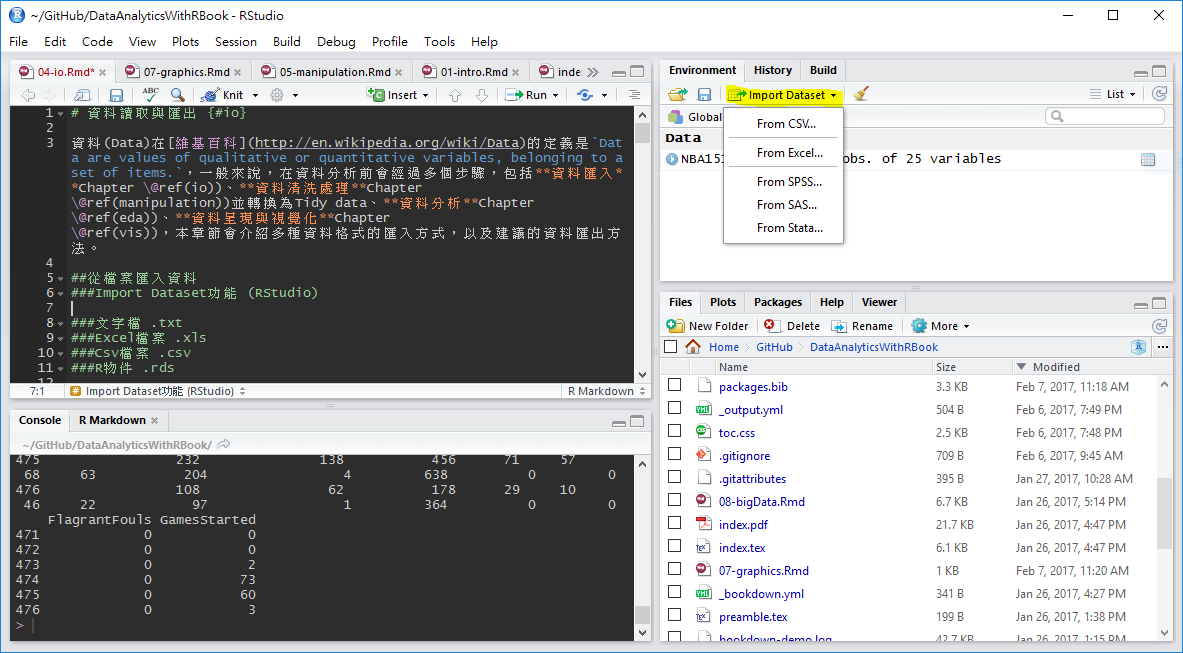
\includegraphics[width=16.43in]{figure/import}

以csv檔案為例,在選單中選取\texttt{From\ CSV},選取後會跳出資料匯入輔助視窗,點選\texttt{Browse}按鈕開啟檔案選取器,並點選欲匯入之文字檔案

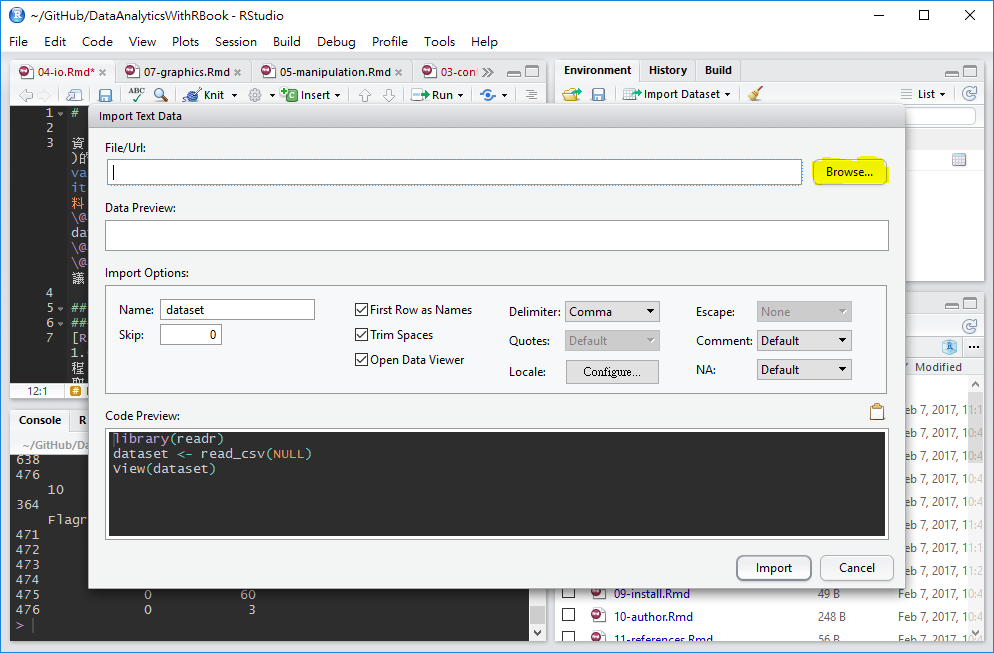
\includegraphics[width=13.81in]{figure/csv}

檔案選取後,資料匯入輔助視窗有預覽功能,供使用者檢查資料匯入方法是否正確,若需調整各項參數,可利用下方\texttt{Import\ Options}的選項微調,最常用的調整功能是\texttt{Delimiter}分隔符號與\texttt{First\ Row\ as\ Names}首列是否為欄位名稱。

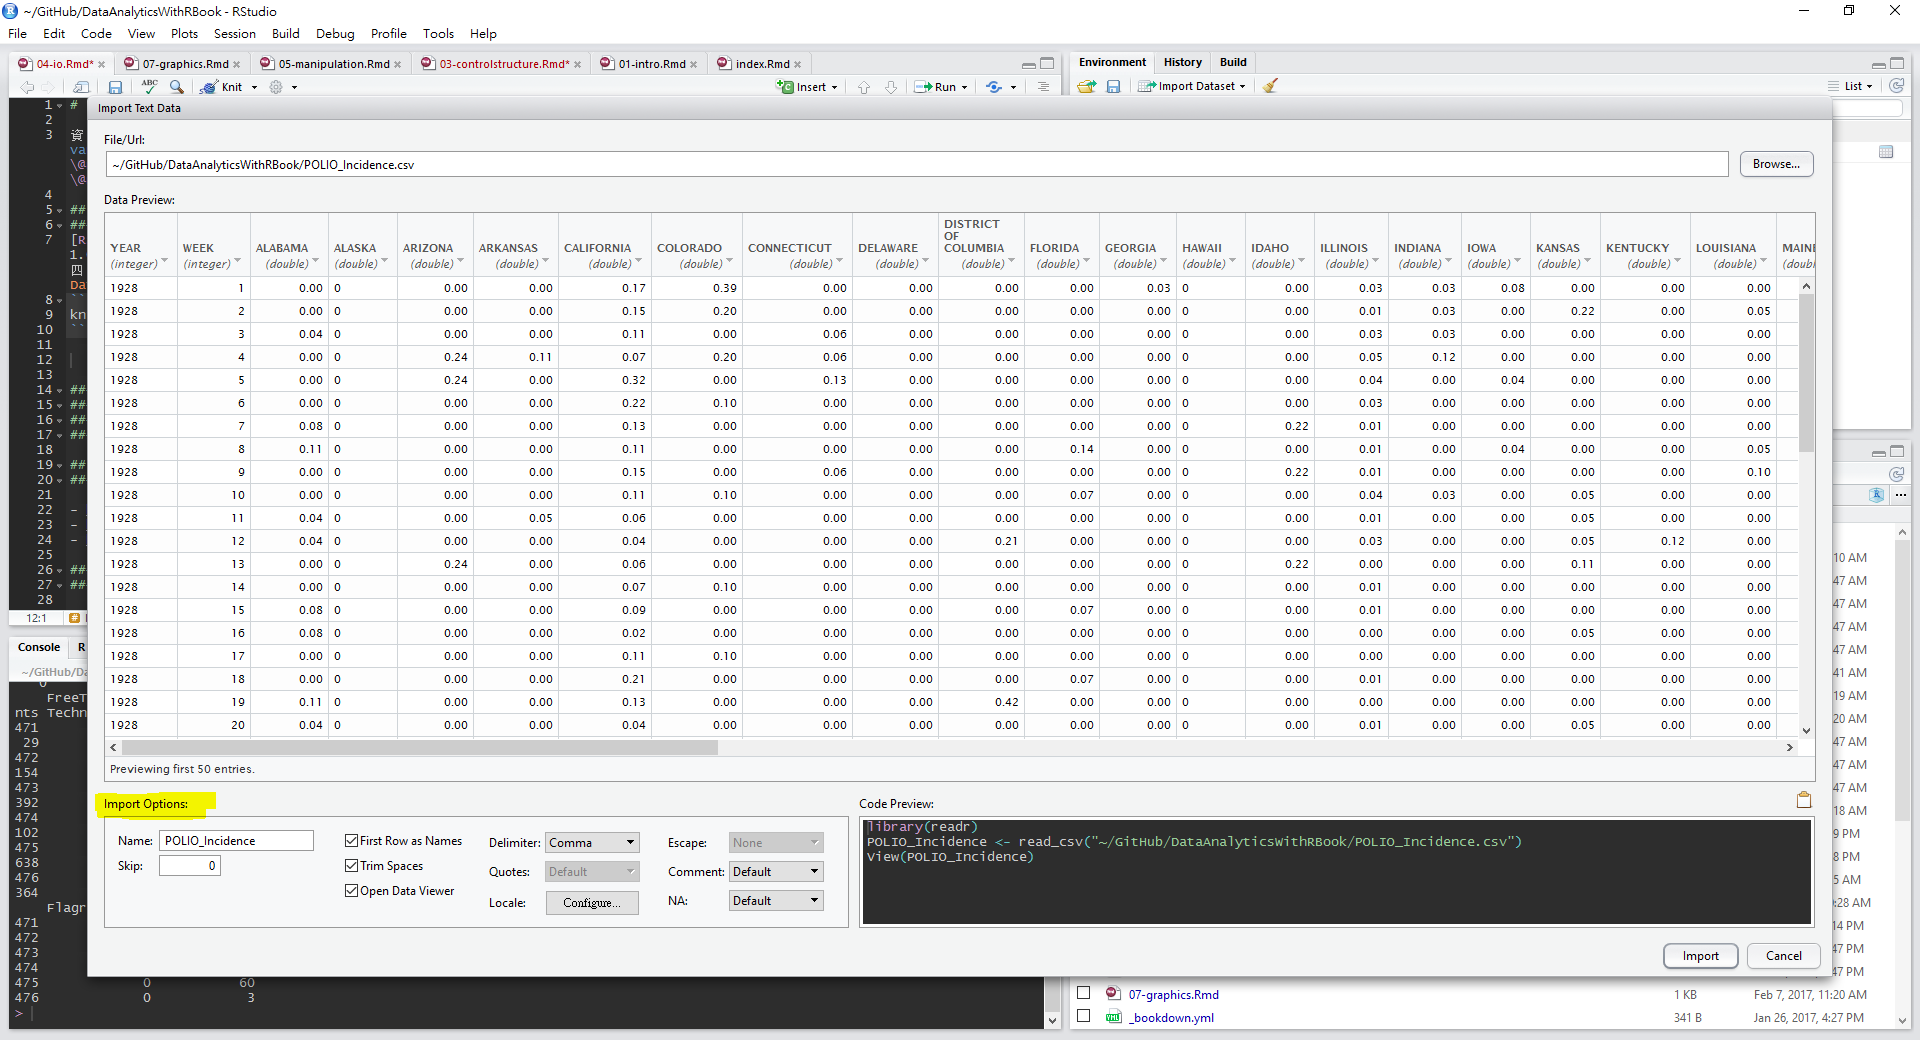
\includegraphics[width=26.67in]{figure/csv2}

如果要匯入的檔案為\textbf{tab分隔文字檔},一樣可以選擇\texttt{.csv}選項,再修改\texttt{Delimiter}參數為\texttt{Tab}即可。

資料匯入輔助視窗右下方\texttt{Code\ Preview:}子視窗中會自動產生資料匯入程式碼,如果未來想再使用視窗匯入,希望透過程式碼匯入,可以將此段程式碼複製貼上到R程式碼檔案(.R),供後續分析使用。

\subsection{分隔文字檔 .txt}\label{-.txt}

\texttt{readr} \citep{R-readr}
package提供完整的文字檔讀取功能,各讀取函數的第一個參數通常為\textbf{檔案路徑與名稱},\texttt{read\_delim()}函數可用來讀取所有用分隔符號分隔的文字檔案,以tab分隔為例,只需將\texttt{delim}參數設定為\texttt{\textbackslash{}t},即可用tab將各欄位分開讀取。此外,\texttt{col\_names}參數也常被使用,TRUE代表資料內有包含欄位名稱(通常在首列),預設為TRUE,如果設定為FALSE,欄位名稱則會一順序被設定為
X1, X2, X3 \ldots{}。

參數整理如下 (可用?read\_delim指令閱讀官方說明):

\begin{itemize}
\tightlist
\item
  \texttt{file}, 檔名
\item
  \texttt{delim}, 分隔符號
\item
  \texttt{quote}, 把欄位包起來的符號
\item
  \texttt{escape\_backslash}, 預設FALSE,是否用/作為逃脫符號
\item
  \texttt{escape\_double}, 預設TRUE,是否用quote符號作為逃脫符號
\item
  \texttt{col\_names}, 是否有欄位名稱(表頭)(T/F)
\item
  \texttt{col\_types}, 每一個欄位的類別,用向量表示
\item
  \texttt{comment}, 備註標示符號,在備註標示符號之後的文字不會被讀入
\item
  \texttt{skip}, 要跳過幾行?
\end{itemize}

\begin{Shaded}
\begin{Highlighting}[]
\KeywordTok{library}\NormalTok{(readr)}
\NormalTok{dataset <-}\StringTok{ }\KeywordTok{read_delim}\NormalTok{(}\StringTok{"檔案路徑與名稱"}\NormalTok{, }\DataTypeTok{delim=}\StringTok{"}\CharTok{\textbackslash{}t}\StringTok{"}\NormalTok{)}
\end{Highlighting}
\end{Shaded}

\subsection{CSV檔案 .csv}\label{csv}

\texttt{readr} \citep{R-readr} package也提供CSV
(逗號分隔)檔案的讀取功能,\texttt{read\_csv()}

\begin{Shaded}
\begin{Highlighting}[]
\KeywordTok{library}\NormalTok{(readr)}
\NormalTok{dataset <-}\StringTok{ }\KeywordTok{read_csv}\NormalTok{(}\StringTok{"檔案路徑與名稱"}\NormalTok{)}
\end{Highlighting}
\end{Shaded}

\subsection{Excel檔案 .xls}\label{excel-.xls}

\texttt{readxl} \citep{R-readxl} package提供讀取Excel檔案 (xls,
xlsx)的函數\texttt{read\_excel()},除了常用的\texttt{col\_names}參數外,也可使用\texttt{sheet}參數設定要讀取的工作表(sheet)

\begin{Shaded}
\begin{Highlighting}[]
\KeywordTok{library}\NormalTok{(readxl)}
\NormalTok{dataset <-}\StringTok{ }\KeywordTok{read_excel}\NormalTok{(}\StringTok{"檔案路徑與名稱"}\NormalTok{)}
\end{Highlighting}
\end{Shaded}

\subsection{R物件 .rds}\label{r-.rds}

R物件有檔案小與讀取快速的優點,如果在R程式處理資料後必須儲存一份以供後續分析的話,使用R物件儲存是最佳的方式,讀取R物件有多種函數可供選擇,推薦使用\texttt{readRDS()}函數
(參考資料:\href{http://www.fromthebottomoftheheap.net/2012/04/01/saving-and-loading-r-objects/}{A
better way of saving and loading objects in R})

\begin{Shaded}
\begin{Highlighting}[]
\NormalTok{dataset <-}\StringTok{ }\KeywordTok{readRDS}\NormalTok{(}\StringTok{"檔案路徑與名稱"}\NormalTok{)}
\end{Highlighting}
\end{Shaded}

\subsection{R程式 .R}\label{r-.r}

\texttt{source}, 讀R的Obejct or script, 執行, ASCII
(\texttt{dump}的相反)

\subsection{純文字資料 (無分隔)}\label{-}

\texttt{readLines}, 逐行讀取文字資料

\subsection{其他讀檔注意事項}

讀檔的時候R會自動

\begin{itemize}
\tightlist
\item
  跳過\#開頭的任何行(Row)
\item
  判斷要讀幾行
\item
  判斷每個列(Column)的類別
\item
  把欄位包起來的符號
\end{itemize}

如果讀取時已指定\textbf{Column類別}以及\textbf{把欄位包起來的符號},讀取速度會快很多。

\section{從網路匯入資料}

\subsection{Open Data}\label{open-data}

\textbf{開放資料} (Open data)
指的是一種經過挑選與許可的資料,這些資料不受著作權、專利權,以及其他管理機制所限制,可以開放給社會公眾,任何人都可以自由出版使用,不論是要拿來出版或是做其他的運用都不加以限制。Open
data
運動希望達成的目標與開放原始碼、內容開放、開放獲取等其他「開放」運動類似。Open
data 背後的核心思想由來已,但 Open data
這名詞直到近代才出現,拜網際網路崛起而為人所知,尤其是 Data.gov 等 Open
data
政府組織的設立。\href{https://zh.wikipedia.org/wiki/\%E9\%96\%8B\%E6\%94\%BE\%E8\%B3\%87\%E6\%96\%99}{維基百科}

台灣政府從2011年開始大力推動開放政府與開放資料的概念,多個機關與縣市政府架設開放資料平台,供民眾擷取或再利用各項資料

\begin{itemize}
\tightlist
\item
  \href{http://data.gov.tw/}{政府資料開放平台}
\item
  \href{http://data.taipei/}{Data Taipei}
\item
  \href{http://data.tycg.gov.tw/}{開放資料 x 開放桃園}
\item
  \href{http://data.moi.gov.tw/}{內政資料開放平台}
\end{itemize}

Open Data常見的儲存方式為: \texttt{CSV}Chapter
\ref{csv}、\texttt{JSON}Chapter \ref{json}、\texttt{XML}Chapter
\ref{xml},開放資料網站通常有提供民眾\textbf{直接下載}檔案的服務,針對可下載的CSV格式資料,可以下載完成後,透過上述\textbf{由檔案匯入資料}
Chapter \ref{file}方法匯入即可。

\subsection{API (Application programming interfaces)}\label{api}

應用程式介面 Application programming interfaces (API)
是軟體系統不同組成部分銜接的約定。由於近年來軟體的規模日益龐大,常常需要把複雜的系統劃分成小的組成部分,編程介面的設計十分重要。程式設計的實踐中,編程介面的設計首先要使軟體系統的職責得到合理劃分。良好的介面設計可以降低系統各部分的相互依賴,提高組成單元的內聚性,降低組成單元間的耦合程度,從而提高系統的維護性和擴充功能性。\href{https://zh.wikipedia.org/zh-tw/\%E5\%BA\%94\%E7\%94\%A8\%E7\%A8\%8B\%E5\%BA\%8F\%E6\%8E\%A5\%E5\%8F\%A3}{Wiki}
但若檔案更新頻繁,以\href{http://data.taipei/opendata/datalist/datasetMeta?oid=6a3e862a-e1cb-4e44-b989-d35609559463}{臺北市開放認養動物}資料資料為例,更新頻率為每日,若使用手動下載相當耗時,所以許多開放資料也提供透過\textbf{API}下載的服務,透過API下載的資料格式會是JSON格式Chapter
\ref{json},如\href{http://data.taipei/opendata/datalist/datasetMeta/outboundDesc?id=6a3e862a-e1cb-4e44-b989-d35609559463\&rid=f4a75ba9-7721-4363-884d-c3820b0b917c}{臺北市開放認養動物API資訊}所示,開放資料網站會提供\textbf{資料集ID}與\textbf{資料RID}

\begin{itemize}
\tightlist
\item
  \textbf{資料集ID}: 紀錄資料的基本參數,如包含欄位、更新頻率等
\item
  \textbf{資料RID}: 資料集
\end{itemize}

並同時提供擷取範例,如果需要下載原始資料,可直接從範例複製貼上即可,如http://data.taipei/opendata/datalist/apiAccess?scope=resourceAquire\&rid=f4a75ba9-7721-4363-884d-c3820b0b917c

\subsection{JSON格式檔案}\label{json}

JSON (\textbf{J}ava\textbf{s}cript \textbf{O}bject
\textbf{N}otation)是一種輕量級的資料交換語言
\href{http://en.wikipedia.org/wiki/JSON}{Wiki},特色如下:

\begin{itemize}
\tightlist
\item
  from \textbf{a}pplication \textbf{p}rogramming \textbf{i}nterfaces
  (APIs)
\item
  JavaScript、Java、Node.js應用
\item
  一些NoSQL非關係型資料庫用JSON儲存格資料:\textbf{MongoDB}
\item
  資料儲存格式

  \begin{itemize}
  \tightlist
  \item
    Numbers (double)
  \item
    Strings (double quoted)
  \item
    Boolean (\emph{true} or \emph{false})
  \item
    Array (ordered, comma separated enclosed in square brackets
    \emph{\protect\hyperlink{preface}{}})
  \item
    Object (unorderd, comma separated collection of \textbf{key:value}
    pairs in curley brackets \emph{\{\}})
  \end{itemize}
\end{itemize}

\href{https://api.github.com/users/yijutseng/repos}{JSON檔案範例}

許多Open
Data也用JSON格式儲存,例如\href{http://data.taipei/opendata/datalist/datasetMeta?oid=6a3e862a-e1cb-4e44-b989-d35609559463}{臺北市開放認養動物}資料,根據資料的API資訊,可得資料擷取網址http://data.taipei/opendata/datalist/apiAccess?scope=resourceAquire\&rid=f4a75ba9-7721-4363-884d-c3820b0b917c
。

將JSON檔案匯入R可以使用\texttt{jsonlite}\citep{R-jsonlite}
package,套件使用前必須安裝,安裝套件方法請參考Chapter
\ref{intro},載入後,可使用\texttt{fromJSON()}函數載入JSON資料。
如需直接從API網址截取資料,需要載入\texttt{RCurl}\citep{R-RCurl}
package,並使用\texttt{getURL()}函數處理資料擷取網址。

\begin{Shaded}
\begin{Highlighting}[]
\KeywordTok{library}\NormalTok{(jsonlite)}
\KeywordTok{library}\NormalTok{(RCurl)}
\NormalTok{PetData<-}\KeywordTok{fromJSON}\NormalTok{(}\KeywordTok{getURL}\NormalTok{(}\StringTok{"http://data.taipei/opendata/datalist/apiAccess?scope=resourceAquire&rid=f4a75ba9-7721-4363-884d-c3820b0b917c"}\NormalTok{))}
\KeywordTok{str}\NormalTok{(PetData)}
\end{Highlighting}
\end{Shaded}

\begin{verbatim}
## List of 1
##  $ result:List of 5
##   ..$ offset : int 0
##   ..$ limit  : int 10000
##   ..$ count  : int 308
##   ..$ sort   : chr ""
##   ..$ results:'data.frame':  308 obs. of  20 variables:
##   .. ..$ _id            : chr [1:308] "1" "2" "3" "4" ...
##   .. ..$ Name           : chr [1:308] "威利" "" "妮妮 " "桔福" ...
##   .. ..$ Sex            : chr [1:308] "雄" "雄" "雌" "雄" ...
##   .. ..$ Type           : chr [1:308] "犬" "貓" "犬" "貓" ...
##   .. ..$ Build          : chr [1:308] "中" "中" "小" "中" ...
##   .. ..$ Age            : chr [1:308] "成年" "老年" "年輕" "成年" ...
##   .. ..$ Variety        : chr [1:308] "米克斯" "米克斯" "米克斯" "米克斯" ...
##   .. ..$ Reason         : chr [1:308] "民眾不擬續養" "民眾拾獲" "民眾不擬續養" "動物管制" ...
##   .. ..$ AcceptNum      : chr [1:308] "106020301" "106012706" "106012601" "106012602" ...
##   .. ..$ ChipNum        : chr [1:308] "965000000263051" "" "900073000086609" "" ...
##   .. ..$ IsSterilization: chr [1:308] "已絕育" "未絕育" "未絕育" "未絕育" ...
##   .. ..$ HairType       : chr [1:308] "黃白" "黃白" "黃" "黃白" ...
##   .. ..$ Note           : chr [1:308] "哈囉~我叫威利,我個性溫馴,但對陌生人有戒心,如果比較靠近可能會有攻擊的行為,所以要先多跟我培養感情唷!!" "疑似高處掉落 疑似無視覺 血尿" "皮膚病\n你好~我的名字叫妮妮,雖然我目前的狀況不太好,但只要好好照顧、增強抵抗力,就可以改善了唷!\n" "臉傷" ...
##   .. ..$ Resettlement   : chr [1:308] "臺北市動物之家 收容編號106020301" "臺北市動物之家 收容編號:106012706" "臺北市動物之家 收容編號106012601" "臺北市動物之家 收容編號:106012602" ...
##   .. ..$ Phone          : chr [1:308] "02-87913062" "02-87913062" "02-87913062" "02-87913062" ...
##   .. ..$ Email          : chr [1:308] "tcapoa8@mail.taipei.gov.tw" "tcapoa8@mail.taipei.gov.tw" "tcapoa8@mail.taipei.gov.tw" "tcapoa8@mail.taipei.gov.tw" ...
##   .. ..$ ChildreAnlong  : chr [1:308] "" "" "" "" ...
##   .. ..$ AnimalAnlong   : chr [1:308] "" "" "" "" ...
##   .. ..$ Bodyweight     : chr [1:308] "" "" "" "" ...
##   .. ..$ ImageName      : chr [1:308] "http://163.29.39.183/uploads/images/medium/6704940d-e354-478f-b136-2f5e167db2fd.jpg" "http://163.29.39.183/uploads/images/medium/e07b5bdb-5138-439d-b83e-9e0347a3cb70.jpg" "http://163.29.39.183/uploads/images/medium/24abcf2b-9b48-43f3-afd8-d027be7de948.jpg" "http://163.29.39.183/uploads/images/medium/af55b5d8-6953-4ec8-9882-b692bf130b81.jpg" ...
\end{verbatim}

由資料結構可知,經過\texttt{fromJSON()}函數匯入的JSON檔案被轉存為\texttt{列表list}的型態,且在result元素中包含五個子元素(offset,
limit, count, sort,
results),其中,results子元素的類別為資料框data.frame,內含開放認養動物清單,因此,可使用\texttt{\$}符號截取元素與子元素

\begin{Shaded}
\begin{Highlighting}[]
\NormalTok{knitr::}\KeywordTok{kable}\NormalTok{(}\KeywordTok{head}\NormalTok{(PetData$result$results)) }
\end{Highlighting}
\end{Shaded}

\begin{tabular}{l|l|l|l|l|l|l|l|l|l|l|l|l|l|l|l|l|l|l|l}
\hline
\_id & Name & Sex & Type & Build & Age & Variety & Reason & AcceptNum & ChipNum & IsSterilization & HairType & Note & Resettlement & Phone & Email & ChildreAnlong & AnimalAnlong & Bodyweight & ImageName\\
\hline
1 & 威利 & 雄 & 犬 & 中 & 成年 & 米克斯 & 民眾不擬續養 & 106020301 & 965000000263051 & 已絕育 & 黃白 & 哈囉\textasciitilde{}我叫威利,我個性溫馴,但對陌生人有戒心,如果比較靠近可能會有攻擊的行為,所以要先多跟我培養感情唷!! & 臺北市動物之家 收容編號106020301 & 02-87913062 & tcapoa8@mail.taipei.gov.tw &  &  &  & http://163.29.39.183/uploads/images/medium/6704940d-e354-478f-b136-2f5e167db2fd.jpg\\
\hline
2 &  & 雄 & 貓 & 中 & 老年 & 米克斯 & 民眾拾獲 & 106012706 &  & 未絕育 & 黃白 & 疑似高處掉落 疑似無視覺 血尿 & 臺北市動物之家 收容編號:106012706 & 02-87913062 & tcapoa8@mail.taipei.gov.tw &  &  &  & http://163.29.39.183/uploads/images/medium/e07b5bdb-5138-439d-b83e-9e0347a3cb70.jpg\\
\hline
3 & 妮妮 & 雌 & 犬 & 小 & 年輕 & 米克斯 & 民眾不擬續養 & 106012601 & 900073000086609 & 未絕育 & 黃 & 皮膚病
你好\textasciitilde{}我的名字叫妮妮,雖然我目前的狀況不太好,但只要好好照顧、增強抵抗力,就可以改善了唷! & 臺北市動物之家 收容編號106012601 & 02-87913062 & tcapoa8@mail.taipei.gov.tw &  &  &  & http://163.29.39.183/uploads/images/medium/24abcf2b-9b48-43f3-afd8-d027be7de948.jpg\\
\hline
4 & 桔福 & 雄 & 貓 & 中 & 成年 & 米克斯 & 動物管制 & 106012602 &  & 未絕育 & 黃白 & 臉傷 & 臺北市動物之家 收容編號:106012602 & 02-87913062 & tcapoa8@mail.taipei.gov.tw &  &  &  & http://163.29.39.183/uploads/images/medium/af55b5d8-6953-4ec8-9882-b692bf130b81.jpg\\
\hline
5 &  & 雄 & 貓 & 大 & 老年 & 米克斯 & 民眾拾獲 & 106012510 &  & 未絕育 & 虎斑白 & 上呼吸道感染 無睪丸 缺右上犬齒 &  &  &  &  &  &  & http://163.29.39.183/uploads/images/medium/411b54ce-59ae-45d5-adcf-d7c5f66ccb86.jpg\\
\hline
6 & Nana & 雌 & 犬 & 中 & 成年 & 米克斯 & 民眾拾獲 & 106012504 &  & 未絕育 & 黑 & 我是Nana
我才剛來動物之家不久
所以還是有些害羞、防備
如果要與我互動記得動作別太大唷
這可是會嚇到我的
希望你們願意花些時間與耐心
慢慢建立起我對你們的信任
來動物之家看看我吧! & 臺北市動物之家 收容編號106012504 & 02-87913062 & tcapoa8@mail.taipei.gov.tw &  &  &  & http://163.29.39.183/uploads/images/medium/9bbf0d11-2dad-4bf6-b732-c0a40f2df146.jpg\\
\hline
\end{tabular}

results資料框中包含20個欄位,可以像分析資料框一樣,針對此資料框做分析,舉例來說,可分析各項\textbf{開放認養理由}出現次數

\begin{Shaded}
\begin{Highlighting}[]
\KeywordTok{table}\NormalTok{(PetData$result$results$Reason)}
\end{Highlighting}
\end{Shaded}

\begin{verbatim}
## 
##              民眾不擬續養     民眾拾獲     動物救援     動物管制 
##           28           41           23          105          111
\end{verbatim}

分析可知開放認養理由以動物管制與未填寫居多。

如果需要將資料框轉換成JSON檔案可以使用\texttt{jsonlite}
package所提供的\texttt{toJSON()}函數。

\begin{Shaded}
\begin{Highlighting}[]
\NormalTok{myjson <-}\StringTok{ }\KeywordTok{toJSON}\NormalTok{(iris, }\DataTypeTok{pretty=}\OtherTok{TRUE}\NormalTok{)}
\KeywordTok{str}\NormalTok{(myjson)}
\end{Highlighting}
\end{Shaded}

\begin{verbatim}
## Class 'json'  chr "[\n  {\n    \"Sepal.Length\": 5.1,\n    \"Sepal.Width\": 3.5,\n    \"Petal.Length\": 1.4,\n    \"Petal.Width\": 0.2,\n    \"Spe"| __truncated__
\end{verbatim}

\subsection{XML 可延伸標記式語言}\label{xml}

\begin{itemize}
\tightlist
\item
  E\textbf{x}tensible \textbf{m}arkup \textbf{l}anguage
\item
  描述\textbf{結構化}資料的語言
\item
  處理XML檔案是網頁\textbf{Html}爬蟲的基礎
\item
  Components

  \begin{itemize}
  \tightlist
  \item
    Markup 標記 - labels that give the text structure
  \item
    Content 內文 - the actual text of the document
  \end{itemize}
\item
  \href{https://zh.wikipedia.org/wiki/XML}{XML Wiki}
\end{itemize}

Tags, elements and attributes

\begin{itemize}
\tightlist
\item
  Tags correspond to general labels

  \begin{itemize}
  \tightlist
  \item
    Start tags \texttt{\textless{}breakfast\_menu\textgreater{}},
    \texttt{\textless{}price\textgreater{}}
  \item
    End tags
    \texttt{\textless{}/breakfast\_menu\textgreater{}},\texttt{\textless{}/price\textgreater{}}
  \item
    Empty tags \texttt{\textless{}line-break\ /\textgreater{}}
  \end{itemize}
\item
  Elements are specific examples of tags

  \begin{itemize}
  \tightlist
  \item
    \texttt{\textless{}name\textgreater{}Belgian\ Waffles\textless{}/name\textgreater{}}
  \end{itemize}
\item
  Attributes are components of the label

  \begin{itemize}
  \tightlist
  \item
    \texttt{\textless{}book\ category="web"\textgreater{}}
  \end{itemize}
\end{itemize}

許多Open
Data也用XML格式儲存,例如\href{http://data.taipei/opendata/datalist/datasetMeta/download?id=961ca397-4a59-45e8-b312-697f26b059dc\&rid=190796c8-7c56-42e0-8068-39242b8ec927}{臺北市水質監測資訊}。如需將XML檔案匯入R中,需要安裝\texttt{XML}
\citep{R-XML} package,使用\texttt{xmlTreeParse()}函數將檔案匯入。

\begin{Shaded}
\begin{Highlighting}[]
\KeywordTok{library}\NormalTok{(XML)}
\NormalTok{waterQ <-}\StringTok{ }\KeywordTok{xmlTreeParse}\NormalTok{(}\StringTok{"http://data.taipei/opendata/datalist/datasetMeta/download?id=961ca397-4a59-45e8-b312-697f26b059dc&rid=190796c8-7c56-42e0-8068-39242b8ec927"}\NormalTok{,}\DataTypeTok{useInternal=}\OtherTok{TRUE}\NormalTok{)}
\NormalTok{rootNode <-}\StringTok{ }\KeywordTok{xmlRoot}\NormalTok{(waterQ) }\CommentTok{#access the top node}
\end{Highlighting}
\end{Shaded}

使用\texttt{xpathSApply()}函數取得指定標籤內的資料

\begin{Shaded}
\begin{Highlighting}[]
\CommentTok{#取得所有"code_name"標籤內的資料}
\KeywordTok{xpathSApply}\NormalTok{(rootNode,}\StringTok{"//code_name"}\NormalTok{,xmlValue)[}\DecValTok{1}\NormalTok{:}\DecValTok{10}\NormalTok{]}
\end{Highlighting}
\end{Shaded}

\begin{verbatim}
##  [1] "雙溪淨水場"               "衛理女中"                
##  [3] "雙溪國小                " "華興加壓站"              
##  [5] "長興淨水場"               "市政大樓"                
##  [7] "市議會"                   "捷運忠孝復興站"          
##  [9] "南港高工"                 "南港加壓站"
\end{verbatim}

\begin{Shaded}
\begin{Highlighting}[]
\CommentTok{#取得各監測站的經度}
\KeywordTok{xpathSApply}\NormalTok{(rootNode,}\StringTok{"//longitude"}\NormalTok{,xmlValue)[}\DecValTok{1}\NormalTok{:}\DecValTok{10}\NormalTok{]}
\end{Highlighting}
\end{Shaded}

\begin{verbatim}
##  [1] "121.56094" "121.54401" "121.55557" "121.53476" "121.54043" "121.55661"
##  [7] "121.55360" "121.53551" "121.59892" "121.60829"
\end{verbatim}

\subsection{網頁爬蟲 Webscraping, Crawling}\label{-webscraping-crawling}

\textbf{Webscraping}: Programatically extracting data from the HTML code
of websites.

\begin{itemize}
\tightlist
\item
  不是每個網站都提供API

  \begin{itemize}
  \tightlist
  \item
    但網頁上卻有你想要分析的資料(像是ptt推文!?)
  \item
    除了人工複製貼上以外,也可以將網頁處理程式化
  \end{itemize}
\item
  可能違法\ldots{}..,一次讀太多太快,很可能被鎖IP
\item
  \href{http://en.wikipedia.org/wiki/Web_scraping}{Webscraping Wiki}
\item
  \href{http://www.largitdata.com/course/1/}{什麼是網頁爬蟲}
\end{itemize}

What's the difference between scraping and crawling

\begin{itemize}
\tightlist
\item
  \texttt{Crawling}

  \begin{itemize}
  \tightlist
  \item
    dealing with \texttt{large\ data-sets} where you develop your own
    crawlers which crawl to the deepest of the \texttt{web\ pages}.
  \end{itemize}
\item
  \texttt{Data\ scraping}

  \begin{itemize}
  \tightlist
  \item
    retrieving information from
    \texttt{any\ source\ (not\ necessarily\ the\ web)}.
  \item
    It's more often the case that irrespective of the approaches
    involved.
  \end{itemize}
\end{itemize}

以\href{http://im.cgu.edu.tw/bin/home.php}{長庚資管系}網站為例,可直接逐行讀取
\texttt{readLines()}

\begin{Shaded}
\begin{Highlighting}[]
\NormalTok{htmlCode <-}\KeywordTok{readLines}\NormalTok{(}\KeywordTok{url}\NormalTok{(}\StringTok{"http://im.cgu.edu.tw/bin/home.php"}\NormalTok{))}
\end{Highlighting}
\end{Shaded}

\begin{verbatim}
## Warning in readLines(url("http://im.cgu.edu.tw/bin/home.php")): 於 'http://
## im.cgu.edu.tw/bin/home.php' 找到不完整的最後一列
\end{verbatim}

\begin{Shaded}
\begin{Highlighting}[]
\NormalTok{htmlCode[}\DecValTok{1}\NormalTok{:}\DecValTok{5}\NormalTok{]}
\end{Highlighting}
\end{Shaded}

\begin{verbatim}
## [1] "<!DOCTYPE html PUBLIC \"-//W3C//DTD XHTML 1.0 Transitional//EN\" \"http://www.w3.org/TR/xhtml1/DTD/xhtml1-transitional.dtd\">"                                                             
## [2] "<html xmlns=\"http://www.w3.org/1999/xhtml\" lang=\"zh-tw\">"                                                                                                                              
## [3] "<head>"                                                                                                                                                                                    
## [4] "<meta http-equiv=\"Content-Type\" content=\"text/html; charset=utf-8\" />"                                                                                                                 
## [5] "<meta http-equiv=\"X-UA-Compatible\" content=\"IE=EmulateIE7\" /><meta name=\"keywords\" content=\"隢‵撖怎雯蝡\x97閮\xba\xbc\xe5\x8d\xa7\u0080\x99\x9f(,)\xe9\x9a\x96\x8b\" />"
\end{verbatim}

用XML工具讀取網頁 (\texttt{XML} package)

\begin{Shaded}
\begin{Highlighting}[]
\KeywordTok{library}\NormalTok{(httr)}
\NormalTok{html <-}\StringTok{ }\KeywordTok{htmlTreeParse}\NormalTok{(}\KeywordTok{GET}\NormalTok{(}\StringTok{"http://im.cgu.edu.tw/bin/home.php"}\NormalTok{), }\DataTypeTok{useInternalNodes=}\NormalTok{T)}
\end{Highlighting}
\end{Shaded}

\begin{verbatim}
## No encoding supplied: defaulting to UTF-8.
\end{verbatim}

\begin{Shaded}
\begin{Highlighting}[]
\KeywordTok{xpathSApply}\NormalTok{(html, }\StringTok{"//title"}\NormalTok{, xmlValue)}
\end{Highlighting}
\end{Shaded}

\begin{verbatim}
## [1] "長庚大學 資訊管理學系 "
\end{verbatim}

\begin{Shaded}
\begin{Highlighting}[]
\KeywordTok{xpathSApply}\NormalTok{(html, }\StringTok{"//span[@class='ptname ']"}\NormalTok{, xmlValue)}
\end{Highlighting}
\end{Shaded}

\begin{verbatim}
##  [1] "畢業專題成果展"       "碩士班計畫書審查"     "畢業校友資料登錄"    
##  [4] "長庚大學首頁"         "校務資訊系統"         "人事教育訓練資訊網"  
##  [7] "國內資管系所"         "碩博士論文網"         "資管系內部行政系統"  
## [10] "資管系分機表"         "資管系學會"           "TA課後輔導值班表"    
## [13] "學生webmail"          "工商管理學系/研究所"  "工業設計學系/研究所" 
## [16] "管理學院"             "醫務管理學系/研究所"  "商管專業學院"        
## [19] "企業管理研究所博士班" "長庚大學行事曆"
\end{verbatim}

其他爬蟲相關參考資源

\begin{itemize}
\tightlist
\item
  R Bloggers
  有很多\href{http://www.r-bloggers.com/?s=Web+Scraping}{爬蟲範例}(英文)
\item
  \href{http://bryannotes.blogspot.tw/2014/08/r-ptt-wantedsocial-network-analysis.html}{Ptt爬蟲實作}
\item
  \href{http://www.largitdata.com/course_list/1}{大數學堂 網頁爬蟲課程}
\end{itemize}

\section{Facebook資料擷取}\label{facebook}

Facebook提供\href{https://developers.facebook.com/docs/graph-api?locale=zh_TW}{Graph
API},讓應用程式可透過API讀取與寫入 Facebook相關資料,\textbf{Graph
API}會根據篩選條件,回傳JSON格式的資料。除此之外,Facebook還提供\href{https://developers.facebook.com/tools/explorer/}{Graph
API Explorer},讓程式開發人員可以測試資料撈取方法和結果。

Get access token

\subsection{Graph API in R}\label{graph-api-in-r}

\begin{Shaded}
\begin{Highlighting}[]
\KeywordTok{library}\NormalTok{(httr)}
\NormalTok{token<-}\StringTok{"your token"} \CommentTok{#將token複製到此處 }
\NormalTok{FBData =}\StringTok{ }\KeywordTok{GET}\NormalTok{(}
    \KeywordTok{paste0}\NormalTok{(}\StringTok{"https://graph.facebook.com/v2.8/tsaiingwen?fields=posts%7Bmessage%7D&access_token="}\NormalTok{,}
           \NormalTok{token))}
\KeywordTok{names}\NormalTok{(FBData)}
\end{Highlighting}
\end{Shaded}

\begin{verbatim}
## [1] "url"         "status_code" "headers"     "all_headers" "cookies"     "content"     "date"       
## [8] "times"       "request"     "handle"    
\end{verbatim}

\begin{Shaded}
\begin{Highlighting}[]
\NormalTok{json1 =}\StringTok{ }\KeywordTok{content}\NormalTok{(FBData)}
\KeywordTok{names}\NormalTok{(json1)}
\end{Highlighting}
\end{Shaded}

\begin{verbatim}
## [1] "posts" "id"
\end{verbatim}

\begin{Shaded}
\begin{Highlighting}[]
\KeywordTok{names}\NormalTok{(json1$posts)}
\end{Highlighting}
\end{Shaded}

\begin{verbatim}
## [1] "data"   "paging"
\end{verbatim}

\begin{Shaded}
\begin{Highlighting}[]
\KeywordTok{head}\NormalTok{(json1$posts$data,}\DecValTok{3}\NormalTok{)}
\end{Highlighting}
\end{Shaded}

\begin{verbatim}
[[1]]
[[1]]$message
[1] "「國機國造」不是夢想,而是一個行動。今天啟動的高級教練機「自研自製」任務,是國防自主的重要里程碑。我們不只要讓戰機起飛,更要讓產業起飛。\n\n國防產業同樣是「5+2」關鍵產業之一,所以,除了要如期、如質完成新式高教機的「自研自製」外,也要重新厚植台灣的航太工業人才鏈,以及加強相關產業的連結、轉型和升級。\n\n國防自主沒有捷徑,只有努力再努力、堅持再堅持。今天,我們重新跨出歷史性的一步。"

[[1]]$id
[1] "46251501064_10154006497451065"


[[2]]
[[2]]$message
[1] "今天,智慧機械推動辦公室正式啟動。「落實產學合作」、「支持創新研發」、「強化行銷通路」是辦公室的三項重點任務。\n\n智慧機械是「5+2」關鍵產業的其中之一。政府有決心。我相信,所有的機械業者-無論做的是螺桿、刀庫、控制器或是工作母機,大家也都有很強的決心,要走向創新、走向智慧化、走向品牌。我們是一個團隊,我們一起加油!"

[[2]]$id
[1] "46251501064_10154006456601065"


[[3]]
[[3]]$message
[1] "今天來向台商拜個晚年。我也邀請台商朋友們,共同參與台灣經濟轉型升級的世紀工程。\n\n無論是擴大對國內的投資,或者配合新南向政策,前進海外深耕佈局,我期待跟台商朋友們一起努力,群策群力,克服困難和瓶頸,為台灣經濟發展打開全新的局面。"

[[3]]$id
[1] "46251501064_10154001652641065"
\end{verbatim}

\begin{Shaded}
\begin{Highlighting}[]
\NormalTok{json1$posts$data[[}\DecValTok{1}\NormalTok{]]$message}
\end{Highlighting}
\end{Shaded}

\begin{verbatim}
##[1] "「國機國造」不是夢想,而是一個行動。今天啟動的高級教練機「自研自製」任務,是國防自主的重要里程碑。我們不只要讓戰機起飛,更要讓產業起飛。\n\n國防產業同樣是「5+2」關鍵產業之一,所以,除了要如期、如質完成新式高教機的「自研自製」外,也要重新厚植台灣的航太工業人才鏈,以及加強相關產業的連結、轉型和升級。\n\n國防自主沒有捷徑,只有努力再努力、堅持再堅持。今天,我們重新跨出歷史性的一步。"
\end{verbatim}

除了直接使用Graph API外,也可使用\texttt{Rfacebook} \citep{R-Rfacebook}
package來讀取Facebook資料

Use Rfacebook To Get Info from \texttt{tsaiingwen} Page

\begin{Shaded}
\begin{Highlighting}[]
\KeywordTok{library}\NormalTok{(Rfacebook)}
\NormalTok{token<-}\StringTok{"your token"} \CommentTok{#將token複製到此處 }
\KeywordTok{getPage}\NormalTok{(}\StringTok{"tsaiingwen"}\NormalTok{, token,}\DataTypeTok{n =} \DecValTok{5}\NormalTok{)}
\end{Highlighting}
\end{Shaded}

\begin{verbatim}
5 posts       from_id           from_name
1 46251501064 蔡英文 Tsai Ing-wen
2 46251501064 蔡英文 Tsai Ing-wen
3 46251501064 蔡英文 Tsai Ing-wen
4 46251501064 蔡英文 Tsai Ing-wen
5 46251501064 蔡英文 Tsai Ing-wen
                                                                                                                                                                                                                                                                                                                                                                                        message
1 「國機國造」不是夢想,而是一個行動。今天啟動的高級教練機「自研自製」任務,是國防自主的重要里程碑。我們不只要讓戰機起飛,更要讓產業起飛。\n\n國防產業同樣是「5+2」關鍵產業之一,所以,除了要如期、如質完成新式高教機的「自研自製」外,也要重新厚植台灣的航太工業人才鏈,以及加強相關產業的連結、轉型和升級。\n\n國防自主沒有捷徑,只有努力再努力、堅持再堅持。今天,我們重新跨出歷史性的一步。
2                                                                   今天,智慧機械推動辦公室正式啟動。「落實產學合作」、「支持創新研發」、「強化行銷通路」是辦公室的三項重點任務。\n\n智慧機械是「5+2」關鍵產業的其中之一。政府有決心。我相信,所有的機械業者-無論做的是螺桿、刀庫、控制器或是工作母機,大家也都有很強的決心,要走向創新、走向智慧化、走向品牌。我們是一個團隊,我們一起加油!
3                                                                                                                                                          今天來向台商拜個晚年。我也邀請台商朋友們,共同參與台灣經濟轉型升級的世紀工程。\n\n無論是擴大對國內的投資,或者配合新南向政策,前進海外深耕佈局,我期待跟台商朋友們一起努力,群策群力,克服困難和瓶頸,為台灣經濟發展打開全新的局面。
4                                                                                                                                                                                                                                                                                    「快了」!雞年通機捷,等待很值得。大年初四,我來看看機場捷運通車前的準備,也坐捷運到中壢,跟鄉親拜年問好。
5                                                                                                                                                                                                                                                                                                            雞年初三發福袋\n\n臺中豐原慈濟宮、彰化溪湖福安宮、雲林北港朝天宮、嘉義九華山地藏庵
              created_time  type
1 2017-02-07T08:02:45+0000 photo
2 2017-02-07T07:18:00+0000 photo
3 2017-02-05T07:12:52+0000 photo
4 2017-01-31T08:37:42+0000 photo
5 2017-01-30T11:41:07+0000 photo
                                                                                                    link
1 https://www.facebook.com/tsaiingwen/photos/a.390960786064.163647.46251501064/10154006497206065/?type=3
2 https://www.facebook.com/tsaiingwen/photos/a.390960786064.163647.46251501064/10154006455396065/?type=3
3 https://www.facebook.com/tsaiingwen/photos/a.390960786064.163647.46251501064/10154001652641065/?type=3
4 https://www.facebook.com/tsaiingwen/photos/a.390960786064.163647.46251501064/10153989357181065/?type=3
5 https://www.facebook.com/tsaiingwen/photos/a.390960786064.163647.46251501064/10153987089121065/?type=3
                             id likes_count comments_count shares_count
1 46251501064_10154006497451065        2013            125           43
2 46251501064_10154006456601065        2217            163           57
3 46251501064_10154001652641065        9416            920          163
4 46251501064_10153989358051065       34116           1574          373
5 46251501064_10153987095776065       20592            665          269
\end{verbatim}

How To Get More Data? Use \textbf{since} and \textbf{until}

Set the dates vector

\begin{Shaded}
\begin{Highlighting}[]
\NormalTok{lastDate<-}\KeywordTok{Sys.Date}\NormalTok{()}
\NormalTok{DateVector<-}\KeywordTok{seq}\NormalTok{(}\KeywordTok{as.Date}\NormalTok{(}\StringTok{"2017-01-01"}\NormalTok{),lastDate,}\DataTypeTok{by=}\StringTok{"5 days"}\NormalTok{)}
\NormalTok{DateVectorStr<-}\KeywordTok{as.character}\NormalTok{(DateVector)}
\NormalTok{DateVectorStr}
\end{Highlighting}
\end{Shaded}

\begin{verbatim}
## "2017-01-01" "2017-01-06" "2017-01-11" "2017-01-16" "2017-01-21" "2017-01-26" "2017-01-31" "2017-02-05"
\end{verbatim}

\begin{Shaded}
\begin{Highlighting}[]
\NormalTok{totalPage<-}\OtherTok{NULL}
\NormalTok{token<-}\StringTok{'your token'}
\NormalTok{numberOfPost<-}\DecValTok{30}
\NormalTok{for(i in }\DecValTok{1}\NormalTok{:(}\KeywordTok{length}\NormalTok{(DateVectorStr)-}\DecValTok{1}\NormalTok{))\{}
    \NormalTok{tempPage<-}\KeywordTok{getPage}\NormalTok{(}\StringTok{"tsaiingwen"}\NormalTok{, token,}
                      \DataTypeTok{since =} \NormalTok{DateVectorStr[i],}\DataTypeTok{until =} \NormalTok{DateVectorStr[i}\DecValTok{+1}\NormalTok{])}
    \NormalTok{totalPage<-}\KeywordTok{rbind}\NormalTok{(totalPage,tempPage)}
\NormalTok{\}}
\KeywordTok{nrow}\NormalTok{(totalPage)}
\end{Highlighting}
\end{Shaded}

\begin{verbatim}
## 4 posts 8 posts 10 posts 3 posts 2 posts 14 posts 1 posts
## [1] 42
\end{verbatim}

Other Useful Methods in Rfacebook Packages

\begin{itemize}
\tightlist
\item
  getUser()
\item
  getPost()
\item
  getLikes()
\item
  Check \url{https://github.com/pablobarbera/Rfacebook}
\item
  ?Rfacebook
\end{itemize}

\section{資料匯出}

在R中完成資料處理後,有多種匯出選擇,如果是要匯出供他人在其他環境(如Excel)使用,建議匯出成tab分隔的文字檔(.txt)或是逗號分隔的文字檔(.csv);但若是要在R的環境繼續使用,建議匯出成R物件
(.rds),除了可保留欄位型別設定外,讀取速度與檔案大小皆優於文字檔案。

\subsection{文字檔 .txt}\label{-.txt}

使用\texttt{write.table()}函數寫入檔案,需要參數有

\begin{itemize}
\tightlist
\item
  \texttt{x} 要匯出的檔案,通常為matrix或是data.frame格式
\item
  \texttt{file} 檔案名稱
\item
  \texttt{append} T/F TRUE表示在檔案後端加入文字,F表示直接覆蓋原始檔案
  (預設F)
\item
  \texttt{quote} 是否需要用雙引號將字串包起 (預設T)
\item
  \texttt{sep} 分隔符號 (預設空白)
\item
  \texttt{eol} 換行符號
\item
  \texttt{na} 表示空值的字串
\item
  \texttt{dec} 小數點表示法
\item
  \texttt{row.names} T/F 是否需要輸出row names
\item
  \texttt{col.names} T/F 是否需要輸出column names
\item
  \texttt{qmethod} 逃脫字串設定
\item
  \texttt{fileEncoding} 編碼設定
\end{itemize}

\begin{Shaded}
\begin{Highlighting}[]
\KeywordTok{write.table}\NormalTok{(iris,}\DataTypeTok{file=}\StringTok{"iris.txt"}\NormalTok{,}\DataTypeTok{sep=}\StringTok{","}\NormalTok{,}\DataTypeTok{row.names =} \NormalTok{F,}\DataTypeTok{col.names =} \NormalTok{T)}
\end{Highlighting}
\end{Shaded}

\subsection{CSV檔 .csv}\label{csv-.csv}

與\texttt{write.table()}類似,使用\texttt{write.csv()}函數寫入檔案

\begin{Shaded}
\begin{Highlighting}[]
\KeywordTok{write.csv}\NormalTok{(iris,}\DataTypeTok{file=}\StringTok{"iris.csv"}\NormalTok{,}\DataTypeTok{row.names =} \NormalTok{F)}
\end{Highlighting}
\end{Shaded}

\subsection{R物件 .rds}\label{r-.rds-1}

若是要在R的環境繼續使用,建議匯出成R物件檔案(.rds)

\begin{Shaded}
\begin{Highlighting}[]
\KeywordTok{saveRDS}\NormalTok{(iris,}\StringTok{"iris.rds"}\NormalTok{)}
\end{Highlighting}
\end{Shaded}

\chapter{資料處理與清洗}\label{manipulation}

\section{Tidy Data}\label{tidy-data}

\begin{itemize}
\tightlist
\item
  一個欄位(Column)內只有一個數值,最好要有凡人看得懂的Column Name
\item
  不同的觀察值應該要在不同行(Raw)
\item
  一張表裡面,有所有分析需要的資料
\item
  如果一定要多張表,中間一定要有index可以把表串起來
\item
  One file, one table
\end{itemize}

\section{資料型別轉換處理}

在資料型態章節Chapter \ref{DataType}中,曾介紹\textbf{數值
(numeric)}、\textbf{字串 (character)}、\textbf{布林變數
(logic)}以及\textbf{日期
(Date)}等資料型態,在此章節中將介紹如何檢查變數型別與各型別的轉換。

\subsection{資料型別檢查}

使用以下\texttt{is.}函數檢查資料型別,回傳布林變數,若為真,回傳TRUE

\begin{itemize}
\tightlist
\item
  是否為\textbf{數字} \texttt{is.numeric(變數名稱)}
\item
  是否為\textbf{文字} \texttt{is.character(變數名稱)}
\item
  是否為\textbf{布林變數} \texttt{is.logical(變數名稱)}
\end{itemize}

\begin{Shaded}
\begin{Highlighting}[]
\NormalTok{num<-}\DecValTok{100}
\NormalTok{cha<-}\StringTok{'200'}
\NormalTok{boo<-T}
\KeywordTok{is.numeric}\NormalTok{(num)}
\end{Highlighting}
\end{Shaded}

\begin{verbatim}
## [1] TRUE
\end{verbatim}

\begin{Shaded}
\begin{Highlighting}[]
\KeywordTok{is.numeric}\NormalTok{(cha)}
\end{Highlighting}
\end{Shaded}

\begin{verbatim}
## [1] FALSE
\end{verbatim}

\begin{Shaded}
\begin{Highlighting}[]
\KeywordTok{is.character}\NormalTok{(num)}
\end{Highlighting}
\end{Shaded}

\begin{verbatim}
## [1] FALSE
\end{verbatim}

\begin{Shaded}
\begin{Highlighting}[]
\KeywordTok{is.character}\NormalTok{(cha)}
\end{Highlighting}
\end{Shaded}

\begin{verbatim}
## [1] TRUE
\end{verbatim}

\begin{Shaded}
\begin{Highlighting}[]
\KeywordTok{is.logical}\NormalTok{(boo)}
\end{Highlighting}
\end{Shaded}

\begin{verbatim}
## [1] TRUE
\end{verbatim}

或使用\texttt{class(變數名稱)}函數,直接回傳資料型別

\begin{Shaded}
\begin{Highlighting}[]
\KeywordTok{class}\NormalTok{(num)}
\end{Highlighting}
\end{Shaded}

\begin{verbatim}
## [1] "numeric"
\end{verbatim}

\begin{Shaded}
\begin{Highlighting}[]
\KeywordTok{class}\NormalTok{(cha)}
\end{Highlighting}
\end{Shaded}

\begin{verbatim}
## [1] "character"
\end{verbatim}

\begin{Shaded}
\begin{Highlighting}[]
\KeywordTok{class}\NormalTok{(boo)}
\end{Highlighting}
\end{Shaded}

\begin{verbatim}
## [1] "logical"
\end{verbatim}

\begin{Shaded}
\begin{Highlighting}[]
\KeywordTok{class}\NormalTok{(}\KeywordTok{Sys.Date}\NormalTok{())}
\end{Highlighting}
\end{Shaded}

\begin{verbatim}
## [1] "Date"
\end{verbatim}

\subsection{資料型別轉換}

使用以下\texttt{as.}函數轉換型別

\begin{itemize}
\tightlist
\item
  轉換為\textbf{數字} \texttt{as.numeric(變數名稱)}
\item
  轉換為\textbf{文字} \texttt{as.character(變數名稱)}
\item
  轉換為\textbf{布林變數} \texttt{as.logical(變數名稱)}
\end{itemize}

\begin{Shaded}
\begin{Highlighting}[]
\KeywordTok{as.numeric}\NormalTok{(cha)}
\end{Highlighting}
\end{Shaded}

\begin{verbatim}
## [1] 200
\end{verbatim}

\begin{Shaded}
\begin{Highlighting}[]
\KeywordTok{as.numeric}\NormalTok{(boo)}
\end{Highlighting}
\end{Shaded}

\begin{verbatim}
## [1] 1
\end{verbatim}

\begin{Shaded}
\begin{Highlighting}[]
\KeywordTok{as.character}\NormalTok{(num)}
\end{Highlighting}
\end{Shaded}

\begin{verbatim}
## [1] "100"
\end{verbatim}

\begin{Shaded}
\begin{Highlighting}[]
\KeywordTok{as.character}\NormalTok{(boo)}
\end{Highlighting}
\end{Shaded}

\begin{verbatim}
## [1] "TRUE"
\end{verbatim}

若無法順利完成轉換,會回傳空值\texttt{NA},並出現警告訊息\texttt{Warning:\ NAs\ introduced\ by\ coercion,Warning:\ 強制變更過程中產生了\ NA}

\begin{Shaded}
\begin{Highlighting}[]
\KeywordTok{as.numeric}\NormalTok{(}\StringTok{"abc"}\NormalTok{)}
\end{Highlighting}
\end{Shaded}

\begin{verbatim}
## Warning: 強制變更過程中產生了 NA
\end{verbatim}

\begin{verbatim}
## [1] NA
\end{verbatim}

日期的轉換則建議使用\texttt{lubridate}\citep{R-lubridate}
package,如果想要將\texttt{年/月/日}格式的文字轉換為日期物件,可使用\texttt{ymd()}函數(y表年year,m表月month,d表日day),如果想要將\texttt{月/日/年}格式的文字轉換為日期物件,則使用\texttt{mdy()}函數,以此類推。

\begin{Shaded}
\begin{Highlighting}[]
\KeywordTok{library}\NormalTok{(lubridate)}
\KeywordTok{ymd}\NormalTok{(}\StringTok{'2012/3/3'}\NormalTok{)}
\end{Highlighting}
\end{Shaded}

\begin{verbatim}
## [1] "2012-03-03"
\end{verbatim}

\begin{Shaded}
\begin{Highlighting}[]
\KeywordTok{mdy}\NormalTok{(}\StringTok{'3/3/2012'}\NormalTok{)}
\end{Highlighting}
\end{Shaded}

\begin{verbatim}
## [1] "2012-03-03"
\end{verbatim}

\section{文字字串處理}

\subsection{基本處理}

\begin{itemize}
\tightlist
\item
  切割 \texttt{strsplit()}
\item
  子集 \texttt{substr()}
\item
  大小寫轉換 \texttt{toupper()} \texttt{tolower()}
\item
  兩文字連接 \texttt{paste()} \texttt{paste0()}
\item
  文字取代 \texttt{gsub()}
\item
  前後空白去除 \texttt{str\_trim()}
  需安裝\texttt{stringr}\citep{R-stringr} package
\end{itemize}

\begin{Shaded}
\begin{Highlighting}[]
\KeywordTok{strsplit} \NormalTok{(}\StringTok{"Hello World"}\NormalTok{,}\StringTok{" "}\NormalTok{)}
\end{Highlighting}
\end{Shaded}

\begin{verbatim}
## [[1]]
## [1] "Hello" "World"
\end{verbatim}

\begin{Shaded}
\begin{Highlighting}[]
\KeywordTok{toupper}\NormalTok{(}\StringTok{"Hello World"}\NormalTok{)}
\end{Highlighting}
\end{Shaded}

\begin{verbatim}
## [1] "HELLO WORLD"
\end{verbatim}

\begin{Shaded}
\begin{Highlighting}[]
\KeywordTok{tolower}\NormalTok{(}\StringTok{"Hello World"}\NormalTok{)}
\end{Highlighting}
\end{Shaded}

\begin{verbatim}
## [1] "hello world"
\end{verbatim}

\begin{Shaded}
\begin{Highlighting}[]
\KeywordTok{paste}\NormalTok{(}\StringTok{"Hello"}\NormalTok{, }\StringTok{"World"}\NormalTok{, }\DataTypeTok{sep=}\StringTok{''}\NormalTok{)}
\end{Highlighting}
\end{Shaded}

\begin{verbatim}
## [1] "HelloWorld"
\end{verbatim}

\begin{Shaded}
\begin{Highlighting}[]
\KeywordTok{substr}\NormalTok{(}\StringTok{"Hello World"}\NormalTok{, }\DataTypeTok{start=}\DecValTok{2}\NormalTok{,}\DataTypeTok{stop=}\DecValTok{4}\NormalTok{)}
\end{Highlighting}
\end{Shaded}

\begin{verbatim}
## [1] "ell"
\end{verbatim}

\begin{Shaded}
\begin{Highlighting}[]
\KeywordTok{gsub}\NormalTok{(}\StringTok{"o"}\NormalTok{,}\StringTok{"0"}\NormalTok{,}\StringTok{"Hello World"}\NormalTok{)}
\end{Highlighting}
\end{Shaded}

\begin{verbatim}
## [1] "Hell0 W0rld"
\end{verbatim}

\begin{Shaded}
\begin{Highlighting}[]
\KeywordTok{library}\NormalTok{(stringr)}
\KeywordTok{str_trim}\NormalTok{(}\StringTok{" Hello World "}\NormalTok{)}
\end{Highlighting}
\end{Shaded}

\begin{verbatim}
## [1] "Hello World"
\end{verbatim}

\subsection{搜尋字串}

搜尋字串函數通常使用在\textbf{比對文字向量},文字比對\textbf{有分大小寫},依照回傳值的型態不同,有兩種常用函數,\texttt{grep()}與\texttt{grepl()}:

\begin{itemize}
\tightlist
\item
  回傳符合條件之向量位置(index) \texttt{grep(搜尋條件,要搜尋的向量)}
\item
  回傳每個向量是否符合條件(TRUE or FALSE)
  \texttt{grepl(搜尋條件,要搜尋的向量)}
\end{itemize}

\begin{Shaded}
\begin{Highlighting}[]
\KeywordTok{grep}\NormalTok{(}\StringTok{"A"}\NormalTok{,}\KeywordTok{c}\NormalTok{(}\StringTok{"Alex"}\NormalTok{,}\StringTok{"Tom"}\NormalTok{,}\StringTok{"Amy"}\NormalTok{,}\StringTok{"Joy"}\NormalTok{,}\StringTok{"Emma"}\NormalTok{)) ##在姓名文字向量中尋找A,回傳包含"A"之元素位置}
\end{Highlighting}
\end{Shaded}

\begin{verbatim}
## [1] 1 3
\end{verbatim}

\begin{Shaded}
\begin{Highlighting}[]
\KeywordTok{grepl}\NormalTok{(}\StringTok{"A"}\NormalTok{,}\KeywordTok{c}\NormalTok{(}\StringTok{"Alex"}\NormalTok{,}\StringTok{"Tom"}\NormalTok{,}\StringTok{"Amy"}\NormalTok{,}\StringTok{"Joy"}\NormalTok{,}\StringTok{"Emma"}\NormalTok{)) ##在姓名文字向量中尋找A,回傳各元素是否包含"A"}
\end{Highlighting}
\end{Shaded}

\begin{verbatim}
## [1]  TRUE FALSE  TRUE FALSE FALSE
\end{verbatim}

\begin{Shaded}
\begin{Highlighting}[]
\KeywordTok{grepl}\NormalTok{(}\StringTok{"a"}\NormalTok{,}\KeywordTok{c}\NormalTok{(}\StringTok{"Alex"}\NormalTok{,}\StringTok{"Tom"}\NormalTok{,}\StringTok{"Amy"}\NormalTok{,}\StringTok{"Joy"}\NormalTok{,}\StringTok{"Emma"}\NormalTok{)) ##在姓名文字向量中尋找a,回傳各元素是否包含"a"}
\end{Highlighting}
\end{Shaded}

\begin{verbatim}
## [1] FALSE FALSE FALSE FALSE  TRUE
\end{verbatim}

\section{子集Subset}\label{subset}

\subsection{一維資料 (向量)}\label{-}

在向量章節\texttt{\{\#vector\}}有介紹使用\texttt{{[}{]}}取出單一或多個元素的方法

\begin{Shaded}
\begin{Highlighting}[]
\NormalTok{letters ##R語言內建資料之一}
\end{Highlighting}
\end{Shaded}

\begin{verbatim}
##  [1] "a" "b" "c" "d" "e" "f" "g" "h" "i" "j" "k" "l" "m" "n" "o" "p" "q" "r" "s"
## [20] "t" "u" "v" "w" "x" "y" "z"
\end{verbatim}

\begin{Shaded}
\begin{Highlighting}[]
\NormalTok{letters[}\DecValTok{1}\NormalTok{] ##取出letters向量的第一個元素}
\end{Highlighting}
\end{Shaded}

\begin{verbatim}
## [1] "a"
\end{verbatim}

\begin{Shaded}
\begin{Highlighting}[]
\NormalTok{letters[}\DecValTok{1}\NormalTok{:}\DecValTok{10}\NormalTok{] ##取出letters向量的前十個元素}
\end{Highlighting}
\end{Shaded}

\begin{verbatim}
##  [1] "a" "b" "c" "d" "e" "f" "g" "h" "i" "j"
\end{verbatim}

\begin{Shaded}
\begin{Highlighting}[]
\NormalTok{letters[}\KeywordTok{c}\NormalTok{(}\DecValTok{1}\NormalTok{,}\DecValTok{3}\NormalTok{,}\DecValTok{5}\NormalTok{)] ##取出letters向量的第1,3,5個元素}
\end{Highlighting}
\end{Shaded}

\begin{verbatim}
## [1] "a" "c" "e"
\end{verbatim}

\begin{Shaded}
\begin{Highlighting}[]
\NormalTok{letters[}\KeywordTok{c}\NormalTok{(-}\DecValTok{1}\NormalTok{,-}\DecValTok{3}\NormalTok{,-}\DecValTok{5}\NormalTok{)] ##取出letters向量除了第1,3,5個元素之外的所有元素}
\end{Highlighting}
\end{Shaded}

\begin{verbatim}
##  [1] "b" "d" "f" "g" "h" "i" "j" "k" "l" "m" "n" "o" "p" "q" "r" "s" "t" "u" "v"
## [20] "w" "x" "y" "z"
\end{verbatim}

若想要快速取得一向量的開頭與結尾元素,可使用\texttt{head()}和\texttt{tail()}函數

\begin{Shaded}
\begin{Highlighting}[]
\KeywordTok{head}\NormalTok{(letters,}\DecValTok{5}\NormalTok{) ##取出letters向量的前五個元素}
\end{Highlighting}
\end{Shaded}

\begin{verbatim}
## [1] "a" "b" "c" "d" "e"
\end{verbatim}

\begin{Shaded}
\begin{Highlighting}[]
\KeywordTok{tail}\NormalTok{(letters,}\DecValTok{3}\NormalTok{) ##取出letters向量的後三個元素}
\end{Highlighting}
\end{Shaded}

\begin{verbatim}
## [1] "x" "y" "z"
\end{verbatim}

\subsection{二維資料}

最常見的二維資料為data.frame資料框,二維資料可針對列(Row)和行(Column)做子集,子集選擇方式一樣是使用\texttt{{[}{]}},但因應二維資料的需求,以\texttt{,}分隔列與行的篩選條件,資料篩選原則為\textbf{前Row,後Column},\textbf{前列,後行},若不想篩選列,則在\texttt{,}前方保持\textbf{空白}即可。

篩選方式可輸入位置(index)、欄位名稱或輸入布林變數(TRUE/FALSE)

\begin{itemize}
\tightlist
\item
  輸入位置: \texttt{dataFrame{[}row\ index,column\ index{]}}
\item
  輸入布林變數: \texttt{dataFrame{[}c(T,F,T),c(T,F,T){]}}
\item
  輸入欄位名稱: \texttt{dataFrame{[}row\ name,column\ name{]}}
\end{itemize}

\begin{Shaded}
\begin{Highlighting}[]
\NormalTok{iris[}\DecValTok{1}\NormalTok{,}\DecValTok{2}\NormalTok{] ##第一列Row,第二行Column}
\end{Highlighting}
\end{Shaded}

\begin{verbatim}
## [1] 3.5
\end{verbatim}

\begin{Shaded}
\begin{Highlighting}[]
\NormalTok{iris[}\DecValTok{1}\NormalTok{:}\DecValTok{3}\NormalTok{,] ##第1~3列Row,所有的行Column}
\end{Highlighting}
\end{Shaded}

\begin{verbatim}
##   Sepal.Length Sepal.Width Petal.Length Petal.Width Species
## 1          5.1         3.5          1.4         0.2  setosa
## 2          4.9         3.0          1.4         0.2  setosa
## 3          4.7         3.2          1.3         0.2  setosa
\end{verbatim}

\begin{Shaded}
\begin{Highlighting}[]
\NormalTok{iris[,}\StringTok{"Species"}\NormalTok{] ##所有的列Row,名稱為Species的行Column}
\end{Highlighting}
\end{Shaded}

\begin{verbatim}
##   [1] setosa     setosa     setosa     setosa     setosa     setosa    
##   [7] setosa     setosa     setosa     setosa     setosa     setosa    
##  [13] setosa     setosa     setosa     setosa     setosa     setosa    
##  [19] setosa     setosa     setosa     setosa     setosa     setosa    
##  [25] setosa     setosa     setosa     setosa     setosa     setosa    
##  [31] setosa     setosa     setosa     setosa     setosa     setosa    
##  [37] setosa     setosa     setosa     setosa     setosa     setosa    
##  [43] setosa     setosa     setosa     setosa     setosa     setosa    
##  [49] setosa     setosa     versicolor versicolor versicolor versicolor
##  [55] versicolor versicolor versicolor versicolor versicolor versicolor
##  [61] versicolor versicolor versicolor versicolor versicolor versicolor
##  [67] versicolor versicolor versicolor versicolor versicolor versicolor
##  [73] versicolor versicolor versicolor versicolor versicolor versicolor
##  [79] versicolor versicolor versicolor versicolor versicolor versicolor
##  [85] versicolor versicolor versicolor versicolor versicolor versicolor
##  [91] versicolor versicolor versicolor versicolor versicolor versicolor
##  [97] versicolor versicolor versicolor versicolor virginica  virginica 
## [103] virginica  virginica  virginica  virginica  virginica  virginica 
## [109] virginica  virginica  virginica  virginica  virginica  virginica 
## [115] virginica  virginica  virginica  virginica  virginica  virginica 
## [121] virginica  virginica  virginica  virginica  virginica  virginica 
## [127] virginica  virginica  virginica  virginica  virginica  virginica 
## [133] virginica  virginica  virginica  virginica  virginica  virginica 
## [139] virginica  virginica  virginica  virginica  virginica  virginica 
## [145] virginica  virginica  virginica  virginica  virginica  virginica 
## Levels: setosa versicolor virginica
\end{verbatim}

\begin{Shaded}
\begin{Highlighting}[]
\NormalTok{iris[}\DecValTok{1}\NormalTok{:}\DecValTok{10}\NormalTok{,}\KeywordTok{c}\NormalTok{(T,F,T,F,T)] ##第1~10列Row,第1,3,5行Column (TRUE)}
\end{Highlighting}
\end{Shaded}

\begin{verbatim}
##    Sepal.Length Petal.Length Species
## 1           5.1          1.4  setosa
## 2           4.9          1.4  setosa
## 3           4.7          1.3  setosa
## 4           4.6          1.5  setosa
## 5           5.0          1.4  setosa
## 6           5.4          1.7  setosa
## 7           4.6          1.4  setosa
## 8           5.0          1.5  setosa
## 9           4.4          1.4  setosa
## 10          4.9          1.5  setosa
\end{verbatim}

也可使用\texttt{\$}符號做\textbf{Column的篩選}

\begin{Shaded}
\begin{Highlighting}[]
\NormalTok{iris$Species ##所有的列Row,名稱為Species的行Column}
\end{Highlighting}
\end{Shaded}

\begin{verbatim}
##   [1] setosa     setosa     setosa     setosa     setosa     setosa    
##   [7] setosa     setosa     setosa     setosa     setosa     setosa    
##  [13] setosa     setosa     setosa     setosa     setosa     setosa    
##  [19] setosa     setosa     setosa     setosa     setosa     setosa    
##  [25] setosa     setosa     setosa     setosa     setosa     setosa    
##  [31] setosa     setosa     setosa     setosa     setosa     setosa    
##  [37] setosa     setosa     setosa     setosa     setosa     setosa    
##  [43] setosa     setosa     setosa     setosa     setosa     setosa    
##  [49] setosa     setosa     versicolor versicolor versicolor versicolor
##  [55] versicolor versicolor versicolor versicolor versicolor versicolor
##  [61] versicolor versicolor versicolor versicolor versicolor versicolor
##  [67] versicolor versicolor versicolor versicolor versicolor versicolor
##  [73] versicolor versicolor versicolor versicolor versicolor versicolor
##  [79] versicolor versicolor versicolor versicolor versicolor versicolor
##  [85] versicolor versicolor versicolor versicolor versicolor versicolor
##  [91] versicolor versicolor versicolor versicolor versicolor versicolor
##  [97] versicolor versicolor versicolor versicolor virginica  virginica 
## [103] virginica  virginica  virginica  virginica  virginica  virginica 
## [109] virginica  virginica  virginica  virginica  virginica  virginica 
## [115] virginica  virginica  virginica  virginica  virginica  virginica 
## [121] virginica  virginica  virginica  virginica  virginica  virginica 
## [127] virginica  virginica  virginica  virginica  virginica  virginica 
## [133] virginica  virginica  virginica  virginica  virginica  virginica 
## [139] virginica  virginica  virginica  virginica  virginica  virginica 
## [145] virginica  virginica  virginica  virginica  virginica  virginica 
## Levels: setosa versicolor virginica
\end{verbatim}

\textbf{Row的篩選}可使用\texttt{subset()}函數,使用方法為\texttt{subset(資料表,篩選邏輯)}

\begin{Shaded}
\begin{Highlighting}[]
\KeywordTok{subset}\NormalTok{(iris,Species==}\StringTok{"virginica"}\NormalTok{) ##Species等於"virginica"的列Row,所有的行Column}
\end{Highlighting}
\end{Shaded}

\begin{verbatim}
##     Sepal.Length Sepal.Width Petal.Length Petal.Width   Species
## 101          6.3         3.3          6.0         2.5 virginica
## 102          5.8         2.7          5.1         1.9 virginica
## 103          7.1         3.0          5.9         2.1 virginica
## 104          6.3         2.9          5.6         1.8 virginica
## 105          6.5         3.0          5.8         2.2 virginica
## 106          7.6         3.0          6.6         2.1 virginica
## 107          4.9         2.5          4.5         1.7 virginica
## 108          7.3         2.9          6.3         1.8 virginica
## 109          6.7         2.5          5.8         1.8 virginica
## 110          7.2         3.6          6.1         2.5 virginica
## 111          6.5         3.2          5.1         2.0 virginica
## 112          6.4         2.7          5.3         1.9 virginica
## 113          6.8         3.0          5.5         2.1 virginica
## 114          5.7         2.5          5.0         2.0 virginica
## 115          5.8         2.8          5.1         2.4 virginica
## 116          6.4         3.2          5.3         2.3 virginica
## 117          6.5         3.0          5.5         1.8 virginica
## 118          7.7         3.8          6.7         2.2 virginica
## 119          7.7         2.6          6.9         2.3 virginica
## 120          6.0         2.2          5.0         1.5 virginica
## 121          6.9         3.2          5.7         2.3 virginica
## 122          5.6         2.8          4.9         2.0 virginica
## 123          7.7         2.8          6.7         2.0 virginica
## 124          6.3         2.7          4.9         1.8 virginica
## 125          6.7         3.3          5.7         2.1 virginica
## 126          7.2         3.2          6.0         1.8 virginica
## 127          6.2         2.8          4.8         1.8 virginica
## 128          6.1         3.0          4.9         1.8 virginica
## 129          6.4         2.8          5.6         2.1 virginica
## 130          7.2         3.0          5.8         1.6 virginica
## 131          7.4         2.8          6.1         1.9 virginica
## 132          7.9         3.8          6.4         2.0 virginica
## 133          6.4         2.8          5.6         2.2 virginica
## 134          6.3         2.8          5.1         1.5 virginica
## 135          6.1         2.6          5.6         1.4 virginica
## 136          7.7         3.0          6.1         2.3 virginica
## 137          6.3         3.4          5.6         2.4 virginica
## 138          6.4         3.1          5.5         1.8 virginica
## 139          6.0         3.0          4.8         1.8 virginica
## 140          6.9         3.1          5.4         2.1 virginica
## 141          6.7         3.1          5.6         2.4 virginica
## 142          6.9         3.1          5.1         2.3 virginica
## 143          5.8         2.7          5.1         1.9 virginica
## 144          6.8         3.2          5.9         2.3 virginica
## 145          6.7         3.3          5.7         2.5 virginica
## 146          6.7         3.0          5.2         2.3 virginica
## 147          6.3         2.5          5.0         1.9 virginica
## 148          6.5         3.0          5.2         2.0 virginica
## 149          6.2         3.4          5.4         2.3 virginica
## 150          5.9         3.0          5.1         1.8 virginica
\end{verbatim}

\textbf{Row的篩選}也可搭配字串搜尋函數\texttt{grepl()}

\begin{Shaded}
\begin{Highlighting}[]
\NormalTok{knitr::}\KeywordTok{kable}\NormalTok{(iris[}\KeywordTok{grepl}\NormalTok{(}\StringTok{"color"}\NormalTok{,iris$Species),]) ##Species包含"color"的列,所有的行}
\end{Highlighting}
\end{Shaded}

\begin{tabular}{l|r|r|r|r|l}
\hline
  & Sepal.Length & Sepal.Width & Petal.Length & Petal.Width & Species\\
\hline
51 & 7.0 & 3.2 & 4.7 & 1.4 & versicolor\\
\hline
52 & 6.4 & 3.2 & 4.5 & 1.5 & versicolor\\
\hline
53 & 6.9 & 3.1 & 4.9 & 1.5 & versicolor\\
\hline
54 & 5.5 & 2.3 & 4.0 & 1.3 & versicolor\\
\hline
55 & 6.5 & 2.8 & 4.6 & 1.5 & versicolor\\
\hline
56 & 5.7 & 2.8 & 4.5 & 1.3 & versicolor\\
\hline
57 & 6.3 & 3.3 & 4.7 & 1.6 & versicolor\\
\hline
58 & 4.9 & 2.4 & 3.3 & 1.0 & versicolor\\
\hline
59 & 6.6 & 2.9 & 4.6 & 1.3 & versicolor\\
\hline
60 & 5.2 & 2.7 & 3.9 & 1.4 & versicolor\\
\hline
61 & 5.0 & 2.0 & 3.5 & 1.0 & versicolor\\
\hline
62 & 5.9 & 3.0 & 4.2 & 1.5 & versicolor\\
\hline
63 & 6.0 & 2.2 & 4.0 & 1.0 & versicolor\\
\hline
64 & 6.1 & 2.9 & 4.7 & 1.4 & versicolor\\
\hline
65 & 5.6 & 2.9 & 3.6 & 1.3 & versicolor\\
\hline
66 & 6.7 & 3.1 & 4.4 & 1.4 & versicolor\\
\hline
67 & 5.6 & 3.0 & 4.5 & 1.5 & versicolor\\
\hline
68 & 5.8 & 2.7 & 4.1 & 1.0 & versicolor\\
\hline
69 & 6.2 & 2.2 & 4.5 & 1.5 & versicolor\\
\hline
70 & 5.6 & 2.5 & 3.9 & 1.1 & versicolor\\
\hline
71 & 5.9 & 3.2 & 4.8 & 1.8 & versicolor\\
\hline
72 & 6.1 & 2.8 & 4.0 & 1.3 & versicolor\\
\hline
73 & 6.3 & 2.5 & 4.9 & 1.5 & versicolor\\
\hline
74 & 6.1 & 2.8 & 4.7 & 1.2 & versicolor\\
\hline
75 & 6.4 & 2.9 & 4.3 & 1.3 & versicolor\\
\hline
76 & 6.6 & 3.0 & 4.4 & 1.4 & versicolor\\
\hline
77 & 6.8 & 2.8 & 4.8 & 1.4 & versicolor\\
\hline
78 & 6.7 & 3.0 & 5.0 & 1.7 & versicolor\\
\hline
79 & 6.0 & 2.9 & 4.5 & 1.5 & versicolor\\
\hline
80 & 5.7 & 2.6 & 3.5 & 1.0 & versicolor\\
\hline
81 & 5.5 & 2.4 & 3.8 & 1.1 & versicolor\\
\hline
82 & 5.5 & 2.4 & 3.7 & 1.0 & versicolor\\
\hline
83 & 5.8 & 2.7 & 3.9 & 1.2 & versicolor\\
\hline
84 & 6.0 & 2.7 & 5.1 & 1.6 & versicolor\\
\hline
85 & 5.4 & 3.0 & 4.5 & 1.5 & versicolor\\
\hline
86 & 6.0 & 3.4 & 4.5 & 1.6 & versicolor\\
\hline
87 & 6.7 & 3.1 & 4.7 & 1.5 & versicolor\\
\hline
88 & 6.3 & 2.3 & 4.4 & 1.3 & versicolor\\
\hline
89 & 5.6 & 3.0 & 4.1 & 1.3 & versicolor\\
\hline
90 & 5.5 & 2.5 & 4.0 & 1.3 & versicolor\\
\hline
91 & 5.5 & 2.6 & 4.4 & 1.2 & versicolor\\
\hline
92 & 6.1 & 3.0 & 4.6 & 1.4 & versicolor\\
\hline
93 & 5.8 & 2.6 & 4.0 & 1.2 & versicolor\\
\hline
94 & 5.0 & 2.3 & 3.3 & 1.0 & versicolor\\
\hline
95 & 5.6 & 2.7 & 4.2 & 1.3 & versicolor\\
\hline
96 & 5.7 & 3.0 & 4.2 & 1.2 & versicolor\\
\hline
97 & 5.7 & 2.9 & 4.2 & 1.3 & versicolor\\
\hline
98 & 6.2 & 2.9 & 4.3 & 1.3 & versicolor\\
\hline
99 & 5.1 & 2.5 & 3.0 & 1.1 & versicolor\\
\hline
100 & 5.7 & 2.8 & 4.1 & 1.3 & versicolor\\
\hline
\end{tabular}

若想要快速取得資料框的前幾列(Raw)或後幾列,也可使用\texttt{head()}和\texttt{tail()}函數

\begin{Shaded}
\begin{Highlighting}[]
\KeywordTok{head}\NormalTok{(iris,}\DecValTok{5}\NormalTok{) ##取出iris資料框的前五列}
\end{Highlighting}
\end{Shaded}

\begin{verbatim}
##   Sepal.Length Sepal.Width Petal.Length Petal.Width Species
## 1          5.1         3.5          1.4         0.2  setosa
## 2          4.9         3.0          1.4         0.2  setosa
## 3          4.7         3.2          1.3         0.2  setosa
## 4          4.6         3.1          1.5         0.2  setosa
## 5          5.0         3.6          1.4         0.2  setosa
\end{verbatim}

\begin{Shaded}
\begin{Highlighting}[]
\KeywordTok{tail}\NormalTok{(iris,}\DecValTok{3}\NormalTok{) ##取出iris資料框的後三列}
\end{Highlighting}
\end{Shaded}

\begin{verbatim}
##     Sepal.Length Sepal.Width Petal.Length Petal.Width   Species
## 148          6.5         3.0          5.2         2.0 virginica
## 149          6.2         3.4          5.4         2.3 virginica
## 150          5.9         3.0          5.1         1.8 virginica
\end{verbatim}

\section{排序}

\subsection{sort 向量排序}\label{sort-}

\texttt{sort()}函數可直接對向量做\textbf{由小到大}的排序

\begin{Shaded}
\begin{Highlighting}[]
\KeywordTok{head}\NormalTok{(islands) ##排序前的前六筆資料}
\end{Highlighting}
\end{Shaded}

\begin{verbatim}
##       Africa   Antarctica         Asia    Australia Axel Heiberg       Baffin 
##        11506         5500        16988         2968           16          184
\end{verbatim}

\begin{Shaded}
\begin{Highlighting}[]
\KeywordTok{head}\NormalTok{(}\KeywordTok{sort}\NormalTok{(islands)) ##由小到大排序後的前六筆資料}
\end{Highlighting}
\end{Shaded}

\begin{verbatim}
##       Vancouver          Hainan Prince of Wales           Timor          Kyushu 
##              12              13              13              13              14 
##          Taiwan 
##              14
\end{verbatim}

如需\textbf{由大到小}排序,可將\texttt{decreasing}參數設為TRUE

\begin{Shaded}
\begin{Highlighting}[]
\KeywordTok{head}\NormalTok{(}\KeywordTok{sort}\NormalTok{(islands,}\DataTypeTok{decreasing =} \NormalTok{T)) ##由大到小排序後的前六筆資料}
\end{Highlighting}
\end{Shaded}

\begin{verbatim}
##          Asia        Africa North America South America    Antarctica 
##         16988         11506          9390          6795          5500 
##        Europe 
##          3745
\end{verbatim}

\subsection{order}\label{order}

如需對資料框做排序,可使用\texttt{order()}函數,\texttt{order()}函數可回傳\textbf{由小到大}之\textbf{元素位置},以\texttt{iris\$Sepal.Length}為例,回傳的第一個位置為\texttt{14},表示\texttt{iris\$Sepal.Length}中,數值最小的元素為第14個元素。

\begin{Shaded}
\begin{Highlighting}[]
\KeywordTok{order}\NormalTok{(iris$Sepal.Length)}
\end{Highlighting}
\end{Shaded}

\begin{verbatim}
##   [1]  14   9  39  43  42   4   7  23  48   3  30  12  13  25  31  46   2  10
##  [19]  35  38  58 107   5   8  26  27  36  41  44  50  61  94   1  18  20  22
##  [37]  24  40  45  47  99  28  29  33  60  49   6  11  17  21  32  85  34  37
##  [55]  54  81  82  90  91  65  67  70  89  95 122  16  19  56  80  96  97 100
##  [73] 114  15  68  83  93 102 115 143  62  71 150  63  79  84  86 120 139  64
##  [91]  72  74  92 128 135  69  98 127 149  57  73  88 101 104 124 134 137 147
## [109]  52  75 112 116 129 133 138  55 105 111 117 148  59  76  66  78  87 109
## [127] 125 141 145 146  77 113 144  53 121 140 142  51 103 110 126 130 108 131
## [145] 106 118 119 123 136 132
\end{verbatim}

\begin{Shaded}
\begin{Highlighting}[]
\NormalTok{iris$Sepal.Length[}\DecValTok{14}\NormalTok{]}
\end{Highlighting}
\end{Shaded}

\begin{verbatim}
## [1] 4.3
\end{verbatim}

若將\texttt{decreasing}參數設定為TRUE,則會回傳\textbf{由大到小}的元素位置,以\texttt{iris\$Sepal.Length}為例,回傳的第一個位置為\texttt{132},表示\texttt{iris\$Sepal.Length}中,數值最大的元素為第132個元素。

\begin{Shaded}
\begin{Highlighting}[]
\KeywordTok{order}\NormalTok{(iris$Sepal.Length,}\DataTypeTok{decreasing =} \NormalTok{T)}
\end{Highlighting}
\end{Shaded}

\begin{verbatim}
##   [1] 132 118 119 123 136 106 131 108 110 126 130 103  51  53 121 140 142  77
##  [19] 113 144  66  78  87 109 125 141 145 146  59  76  55 105 111 117 148  52
##  [37]  75 112 116 129 133 138  57  73  88 101 104 124 134 137 147  69  98 127
##  [55] 149  64  72  74  92 128 135  63  79  84  86 120 139  62  71 150  15  68
##  [73]  83  93 102 115 143  16  19  56  80  96  97 100 114  65  67  70  89  95
##  [91] 122  34  37  54  81  82  90  91   6  11  17  21  32  85  49  28  29  33
## [109]  60   1  18  20  22  24  40  45  47  99   5   8  26  27  36  41  44  50
## [127]  61  94   2  10  35  38  58 107  12  13  25  31  46   3  30   4   7  23
## [145]  48  42   9  39  43  14
\end{verbatim}

\begin{Shaded}
\begin{Highlighting}[]
\NormalTok{iris$Sepal.Length[}\DecValTok{132}\NormalTok{]}
\end{Highlighting}
\end{Shaded}

\begin{verbatim}
## [1] 7.9
\end{verbatim}

依照order回傳的元素位置,重新排序iris資料框

\begin{Shaded}
\begin{Highlighting}[]
\KeywordTok{head}\NormalTok{(iris) ##排序前的前六筆資料}
\end{Highlighting}
\end{Shaded}

\begin{verbatim}
##   Sepal.Length Sepal.Width Petal.Length Petal.Width Species
## 1          5.1         3.5          1.4         0.2  setosa
## 2          4.9         3.0          1.4         0.2  setosa
## 3          4.7         3.2          1.3         0.2  setosa
## 4          4.6         3.1          1.5         0.2  setosa
## 5          5.0         3.6          1.4         0.2  setosa
## 6          5.4         3.9          1.7         0.4  setosa
\end{verbatim}

\begin{Shaded}
\begin{Highlighting}[]
\KeywordTok{head}\NormalTok{(iris[}\KeywordTok{order}\NormalTok{(iris$Sepal.Length),]) ##依照Sepal.Length欄位數值大小排序後的前六筆資料}
\end{Highlighting}
\end{Shaded}

\begin{verbatim}
##    Sepal.Length Sepal.Width Petal.Length Petal.Width Species
## 14          4.3         3.0          1.1         0.1  setosa
## 9           4.4         2.9          1.4         0.2  setosa
## 39          4.4         3.0          1.3         0.2  setosa
## 43          4.4         3.2          1.3         0.2  setosa
## 42          4.5         2.3          1.3         0.3  setosa
## 4           4.6         3.1          1.5         0.2  setosa
\end{verbatim}

\begin{Shaded}
\begin{Highlighting}[]
\KeywordTok{head}\NormalTok{(iris[}\KeywordTok{order}\NormalTok{(iris$Sepal.Length,}\DataTypeTok{decreasing =} \NormalTok{T),]) ##改為由大到小排序的前六筆資料}
\end{Highlighting}
\end{Shaded}

\begin{verbatim}
##     Sepal.Length Sepal.Width Petal.Length Petal.Width   Species
## 132          7.9         3.8          6.4         2.0 virginica
## 118          7.7         3.8          6.7         2.2 virginica
## 119          7.7         2.6          6.9         2.3 virginica
## 123          7.7         2.8          6.7         2.0 virginica
## 136          7.7         3.0          6.1         2.3 virginica
## 106          7.6         3.0          6.6         2.1 virginica
\end{verbatim}

\section{資料組合}

有時需要在資料框新增一列,或新增一行,可以利用資料組合函數完成

\begin{itemize}
\tightlist
\item
  Row 列的組合 \texttt{rbind()}
\item
  Column 行的組合 \texttt{cbind()}
\end{itemize}

\texttt{rbind()}和\texttt{cbind()}的參數可以是向量,也可以是資料框,使用向量做資料整合範例:

\begin{Shaded}
\begin{Highlighting}[]
\KeywordTok{rbind}\NormalTok{(}\KeywordTok{c}\NormalTok{(}\DecValTok{1}\NormalTok{,}\DecValTok{2}\NormalTok{,}\DecValTok{3}\NormalTok{), }\CommentTok{#第一列}
      \KeywordTok{c}\NormalTok{(}\DecValTok{4}\NormalTok{,}\DecValTok{5}\NormalTok{,}\DecValTok{6}\NormalTok{)  }\CommentTok{#第二列}
      \NormalTok{) }
\end{Highlighting}
\end{Shaded}

\begin{verbatim}
##      [,1] [,2] [,3]
## [1,]    1    2    3
## [2,]    4    5    6
\end{verbatim}

使用資料框與向量做資料整合範例:

\begin{Shaded}
\begin{Highlighting}[]
\NormalTok{irisAdd<-}\KeywordTok{rbind}\NormalTok{(iris, }\CommentTok{#資料框}
      \KeywordTok{c}\NormalTok{(}\DecValTok{1}\NormalTok{,}\DecValTok{1}\NormalTok{,}\DecValTok{1}\NormalTok{,}\DecValTok{1}\NormalTok{,}\StringTok{"versicolor"}\NormalTok{)  }\CommentTok{#新增一列}
      \NormalTok{) }
\KeywordTok{tail}\NormalTok{(irisAdd)}
\end{Highlighting}
\end{Shaded}

\begin{verbatim}
##     Sepal.Length Sepal.Width Petal.Length Petal.Width    Species
## 146          6.7           3          5.2         2.3  virginica
## 147          6.3         2.5            5         1.9  virginica
## 148          6.5           3          5.2           2  virginica
## 149          6.2         3.4          5.4         2.3  virginica
## 150          5.9           3          5.1         1.8  virginica
## 151            1           1            1           1 versicolor
\end{verbatim}

使用向量做資料整合範例:

\begin{Shaded}
\begin{Highlighting}[]
\KeywordTok{cbind}\NormalTok{(}\KeywordTok{c}\NormalTok{(}\DecValTok{1}\NormalTok{,}\DecValTok{2}\NormalTok{,}\DecValTok{3}\NormalTok{), }\CommentTok{#第一行}
      \KeywordTok{c}\NormalTok{(}\DecValTok{4}\NormalTok{,}\DecValTok{5}\NormalTok{,}\DecValTok{6}\NormalTok{)  }\CommentTok{#第二行}
      \NormalTok{) }
\end{Highlighting}
\end{Shaded}

\begin{verbatim}
##      [,1] [,2]
## [1,]    1    4
## [2,]    2    5
## [3,]    3    6
\end{verbatim}

使用資料框與向量做資料整合範例:

\begin{Shaded}
\begin{Highlighting}[]
\NormalTok{irisAdd<-}\KeywordTok{cbind}\NormalTok{(iris, }\CommentTok{#資料框}
      \KeywordTok{rep}\NormalTok{(}\StringTok{"Add"}\NormalTok{,}\KeywordTok{nrow}\NormalTok{(iris))  }\CommentTok{#新增一行}
      \NormalTok{) }
\KeywordTok{tail}\NormalTok{(irisAdd)}
\end{Highlighting}
\end{Shaded}

\begin{verbatim}
##     Sepal.Length Sepal.Width Petal.Length Petal.Width   Species
## 145          6.7         3.3          5.7         2.5 virginica
## 146          6.7         3.0          5.2         2.3 virginica
## 147          6.3         2.5          5.0         1.9 virginica
## 148          6.5         3.0          5.2         2.0 virginica
## 149          6.2         3.4          5.4         2.3 virginica
## 150          5.9         3.0          5.1         1.8 virginica
##     rep("Add", nrow(iris))
## 145                    Add
## 146                    Add
## 147                    Add
## 148                    Add
## 149                    Add
## 150                    Add
\end{verbatim}

\section{長表與寬表}

在資料處理的過程中,常因各種需求,需要執行長寬表互換的動作,在R中有很好用的套件reshape2\citep{R-reshape2}
package,提供完整的轉換功能,最常使用的是

\begin{itemize}
\tightlist
\item
  寬表轉長表 \texttt{melt(資料框/寬表,id.vars=需要保留的欄位)}
\item
  長表轉寬表
  \texttt{dcast(資料框/長表,寬表分列依據\textasciitilde{}分欄位依據)}
\end{itemize}

原來的\texttt{airquality}資料框中,有Ozone, Solar.R, Wind, Temp, Month,
Day等六個欄位
(Column),屬於寬表,以下範例將保留Month和Day兩個欄位,並將其他欄位的名稱整合至variable欄位,數值整合至value欄位,寬表轉長表範例如下:

\begin{Shaded}
\begin{Highlighting}[]
\KeywordTok{library}\NormalTok{(reshape2)}
\KeywordTok{head}\NormalTok{(airquality)}
\end{Highlighting}
\end{Shaded}

\begin{verbatim}
##   Ozone Solar.R Wind Temp Month Day
## 1    41     190  7.4   67     5   1
## 2    36     118  8.0   72     5   2
## 3    12     149 12.6   74     5   3
## 4    18     313 11.5   62     5   4
## 5    NA      NA 14.3   56     5   5
## 6    28      NA 14.9   66     5   6
\end{verbatim}

\begin{Shaded}
\begin{Highlighting}[]
\NormalTok{airqualityM<-}\KeywordTok{melt}\NormalTok{(airquality,}\DataTypeTok{id.vars =} \KeywordTok{c}\NormalTok{(}\StringTok{"Month"}\NormalTok{,}\StringTok{"Day"}\NormalTok{)) ##欄位需要保留"Month","Day"}
\KeywordTok{head}\NormalTok{(airqualityM)}
\end{Highlighting}
\end{Shaded}

\begin{verbatim}
##   Month Day variable value
## 1     5   1    Ozone    41
## 2     5   2    Ozone    36
## 3     5   3    Ozone    12
## 4     5   4    Ozone    18
## 5     5   5    Ozone    NA
## 6     5   6    Ozone    28
\end{verbatim}

轉換過的長表\texttt{airqualityM}資料框中,剩下Month, Day, variable,
value等四個欄位
(Column),屬於長表,以下範例variable欄位的值轉換為新欄位,並將value欄位填回新增的欄位,長表轉寬表範例如下:

\begin{Shaded}
\begin{Highlighting}[]
\KeywordTok{library}\NormalTok{(reshape2)}
\NormalTok{##欄位保留"Month","Day"外,其他欄位數目由variable定義}
\NormalTok{airqualityCast<-}\KeywordTok{dcast}\NormalTok{(airqualityM, Month +Day~variable) }
\KeywordTok{head}\NormalTok{(airqualityCast)}
\end{Highlighting}
\end{Shaded}

\begin{verbatim}
##   Month Day Ozone Solar.R Wind Temp
## 1     5   1    41     190  7.4   67
## 2     5   2    36     118  8.0   72
## 3     5   3    12     149 12.6   74
## 4     5   4    18     313 11.5   62
## 5     5   5    NA      NA 14.3   56
## 6     5   6    28      NA 14.9   66
\end{verbatim}

\section{遺漏值處理}

遺漏值(Missing
Value)常常出現在真實資料內,在數值運算時常會有問題,最簡單的方法是將有缺值的資料移除,如資料為向量,可使用\texttt{is.na()}來判斷資料是否為空值\texttt{NA},若為真\texttt{TRUE},則將資料移除。

\begin{Shaded}
\begin{Highlighting}[]
\NormalTok{naVec<-}\KeywordTok{c}\NormalTok{(}\StringTok{"a"}\NormalTok{,}\StringTok{"b"}\NormalTok{,}\OtherTok{NA}\NormalTok{,}\StringTok{"d"}\NormalTok{,}\StringTok{"e"}\NormalTok{)}
\KeywordTok{is.na}\NormalTok{(naVec)}
\end{Highlighting}
\end{Shaded}

\begin{verbatim}
## [1] FALSE FALSE  TRUE FALSE FALSE
\end{verbatim}

\begin{Shaded}
\begin{Highlighting}[]
\NormalTok{naVec[!}\KeywordTok{is.na}\NormalTok{(naVec)] ##保留所有在is.na()檢查回傳FALSE的元素}
\end{Highlighting}
\end{Shaded}

\begin{verbatim}
## [1] "a" "b" "d" "e"
\end{verbatim}

若資料型態為資料框,可使用\texttt{complete.cases}來選出完整的資料列,如果資料列是完整的,則會回傳真TRUE

\begin{Shaded}
\begin{Highlighting}[]
\KeywordTok{head}\NormalTok{(airquality)}
\end{Highlighting}
\end{Shaded}

\begin{verbatim}
##   Ozone Solar.R Wind Temp Month Day
## 1    41     190  7.4   67     5   1
## 2    36     118  8.0   72     5   2
## 3    12     149 12.6   74     5   3
## 4    18     313 11.5   62     5   4
## 5    NA      NA 14.3   56     5   5
## 6    28      NA 14.9   66     5   6
\end{verbatim}

\begin{Shaded}
\begin{Highlighting}[]
\KeywordTok{complete.cases}\NormalTok{(airquality) }
\end{Highlighting}
\end{Shaded}

\begin{verbatim}
##   [1]  TRUE  TRUE  TRUE  TRUE FALSE FALSE  TRUE  TRUE  TRUE FALSE FALSE  TRUE
##  [13]  TRUE  TRUE  TRUE  TRUE  TRUE  TRUE  TRUE  TRUE  TRUE  TRUE  TRUE  TRUE
##  [25] FALSE FALSE FALSE  TRUE  TRUE  TRUE  TRUE FALSE FALSE FALSE FALSE FALSE
##  [37] FALSE  TRUE FALSE  TRUE  TRUE FALSE FALSE  TRUE FALSE FALSE  TRUE  TRUE
##  [49]  TRUE  TRUE  TRUE FALSE FALSE FALSE FALSE FALSE FALSE FALSE FALSE FALSE
##  [61] FALSE  TRUE  TRUE  TRUE FALSE  TRUE  TRUE  TRUE  TRUE  TRUE  TRUE FALSE
##  [73]  TRUE  TRUE FALSE  TRUE  TRUE  TRUE  TRUE  TRUE  TRUE  TRUE FALSE FALSE
##  [85]  TRUE  TRUE  TRUE  TRUE  TRUE  TRUE  TRUE  TRUE  TRUE  TRUE  TRUE FALSE
##  [97] FALSE FALSE  TRUE  TRUE  TRUE FALSE FALSE  TRUE  TRUE  TRUE FALSE  TRUE
## [109]  TRUE  TRUE  TRUE  TRUE  TRUE  TRUE FALSE  TRUE  TRUE  TRUE FALSE  TRUE
## [121]  TRUE  TRUE  TRUE  TRUE  TRUE  TRUE  TRUE  TRUE  TRUE  TRUE  TRUE  TRUE
## [133]  TRUE  TRUE  TRUE  TRUE  TRUE  TRUE  TRUE  TRUE  TRUE  TRUE  TRUE  TRUE
## [145]  TRUE  TRUE  TRUE  TRUE  TRUE FALSE  TRUE  TRUE  TRUE
\end{verbatim}

\begin{Shaded}
\begin{Highlighting}[]
\KeywordTok{head}\NormalTok{(airquality[}\KeywordTok{complete.cases}\NormalTok{(airquality),]) ##保留所有在complete.cases()檢查回傳TRUE的元素}
\end{Highlighting}
\end{Shaded}

\begin{verbatim}
##   Ozone Solar.R Wind Temp Month Day
## 1    41     190  7.4   67     5   1
## 2    36     118  8.0   72     5   2
## 3    12     149 12.6   74     5   3
## 4    18     313 11.5   62     5   4
## 7    23     299  8.6   65     5   7
## 8    19      99 13.8   59     5   8
\end{verbatim}

利用演算法補值也是一種解決辦法,可參考\_skydome20\_的\href{http://www.rpubs.com/skydome20/R-Note10-Missing_Value}{R筆記--(10)遺漏值處理(Impute
Missing Value)}教學。

\section{綜合練習範例}

在本範例中,介紹使用\texttt{SportsAnalytics} \citep{R-SportsAnalytics}
package 撈取NBA各球員的數據,並加以觀察分析。

\subsection{載入資料}

首先用\texttt{library()}函數將\texttt{SportsAnalytics}套件載入
(若尚未安裝此套件者,必須先安裝套件,可參考Chapter
\ref{intro}),並利用套件內提供的\texttt{fetch\_NBAPlayerStatistics()}函數,將對應年份之資料取出。

\begin{Shaded}
\begin{Highlighting}[]
\KeywordTok{library}\NormalTok{(SportsAnalytics)}
\NormalTok{NBA1516<-}\KeywordTok{fetch_NBAPlayerStatistics}\NormalTok{(}\StringTok{"15-16"}\NormalTok{)}
\end{Highlighting}
\end{Shaded}

\subsection{資料總覽}

資料取出後,可用\texttt{str()}函數總覽\texttt{NBA1516}這個資料框的欄位與欄位類別

\begin{Shaded}
\begin{Highlighting}[]
\KeywordTok{str}\NormalTok{(NBA1516)}
\end{Highlighting}
\end{Shaded}

\begin{verbatim}
## 'data.frame':    476 obs. of  25 variables:
##  $ League             : Factor w/ 1 level "NBA": 1 1 1 1 1 1 1 1 1 1 ...
##  $ Name               : chr  "Quincy Acy" "Jordan Adams" "Steven Adams" "Arron Afflalo" ...
##  $ Team               : Factor w/ 31 levels "ATL","BOS","BRO",..: 27 15 22 20 19 13 28 26 12 15 ...
##  $ Position           : Factor w/ 5 levels "C","PF","PG",..: 4 5 1 5 1 1 2 2 2 5 ...
##  $ GamesPlayed        : int  59 2 80 71 59 60 74 9 79 64 ...
##  $ TotalMinutesPlayed : int  877 15 2019 2359 863 802 2260 37 1601 1622 ...
##  $ FieldGoalsMade     : int  119 2 261 354 150 134 536 5 191 215 ...
##  $ FieldGoalsAttempted: int  214 6 426 799 314 225 1045 10 370 469 ...
##  $ ThreesMade         : int  19 0 0 91 0 0 0 0 0 15 ...
##  $ ThreesAttempted    : int  49 1 0 238 1 0 16 0 0 42 ...
##  $ FreeThrowsMade     : int  50 3 114 110 52 60 259 0 46 90 ...
##  $ FreeThrowsAttempted: int  68 5 196 131 62 84 302 0 73 138 ...
##  $ OffensiveRebounds  : int  65 0 218 23 75 86 175 2 162 104 ...
##  $ TotalRebounds      : int  188 2 531 266 269 288 631 6 424 297 ...
##  $ Assists            : int  27 3 61 145 32 50 110 0 76 70 ...
##  $ Steals             : int  29 3 42 25 19 47 38 1 26 109 ...
##  $ Turnovers          : int  27 2 84 82 54 64 99 1 69 78 ...
##  $ Blocks             : int  24 0 89 10 36 68 81 2 42 18 ...
##  $ PersonalFouls      : int  103 2 223 142 134 139 151 1 147 175 ...
##  $ Disqualifications  : int  0 0 2 1 0 1 0 0 1 1 ...
##  $ TotalPoints        : int  307 7 636 909 352 328 1331 10 428 535 ...
##  $ Technicals         : int  3 0 2 1 2 0 0 0 0 1 ...
##  $ Ejections          : int  0 0 0 0 0 0 0 0 0 0 ...
##  $ FlagrantFouls      : int  0 0 0 0 0 0 0 0 0 0 ...
##  $ GamesStarted       : int  29 0 80 57 17 5 74 0 28 56 ...
\end{verbatim}

可以發現此\texttt{NBA1516}資料框內有476筆球員資料(觀察值,
obs),每筆資料有25個欄位 (variables)。 \#\#\#資料預覽
如果想看資料框內容,可用\texttt{head()}和\texttt{tail()}快速瀏覽部分資料

\begin{Shaded}
\begin{Highlighting}[]
\KeywordTok{head}\NormalTok{(NBA1516)}
\end{Highlighting}
\end{Shaded}

\begin{verbatim}
##   League          Name Team Position GamesPlayed TotalMinutesPlayed
## 1    NBA    Quincy Acy  SAC       SF          59                877
## 2    NBA  Jordan Adams  MEM       SG           2                 15
## 3    NBA  Steven Adams  OKL        C          80               2019
## 4    NBA Arron Afflalo  NYK       SG          71               2359
## 5    NBA Alexis Ajinca  NOR        C          59                863
## 6    NBA  Cole Aldrich  LAC        C          60                802
##   FieldGoalsMade FieldGoalsAttempted ThreesMade ThreesAttempted FreeThrowsMade
## 1            119                 214         19              49             50
## 2              2                   6          0               1              3
## 3            261                 426          0               0            114
## 4            354                 799         91             238            110
## 5            150                 314          0               1             52
## 6            134                 225          0               0             60
##   FreeThrowsAttempted OffensiveRebounds TotalRebounds Assists Steals Turnovers
## 1                  68                65           188      27     29        27
## 2                   5                 0             2       3      3         2
## 3                 196               218           531      61     42        84
## 4                 131                23           266     145     25        82
## 5                  62                75           269      32     19        54
## 6                  84                86           288      50     47        64
##   Blocks PersonalFouls Disqualifications TotalPoints Technicals Ejections
## 1     24           103                 0         307          3         0
## 2      0             2                 0           7          0         0
## 3     89           223                 2         636          2         0
## 4     10           142                 1         909          1         0
## 5     36           134                 0         352          2         0
## 6     68           139                 1         328          0         0
##   FlagrantFouls GamesStarted
## 1             0           29
## 2             0            0
## 3             0           80
## 4             0           57
## 5             0           17
## 6             0            5
\end{verbatim}

\subsection{資料排序後篩選}

觀察資料框的組成後,我們想要找出\textbf{出場數}最\textbf{高}的前五名選手的所有資料,此時可以利用\texttt{order()}函數先\textbf{由大到小}排序(\texttt{decreasing\ =\ T})後,再用\texttt{{[},{]}}取子集。

\begin{Shaded}
\begin{Highlighting}[]
\NormalTok{NBA1516Order<-NBA1516[}\KeywordTok{order}\NormalTok{(NBA1516$GamesPlayed,}\DataTypeTok{decreasing =} \NormalTok{T),]}
\NormalTok{NBA1516Order[}\DecValTok{1}\NormalTok{:}\DecValTok{5}\NormalTok{,] ##逗號前方放1~5,表示取1~5列;逗號後方空白,表示要取所有欄位}
\end{Highlighting}
\end{Shaded}

\begin{verbatim}
##     League            Name Team Position GamesPlayed TotalMinutesPlayed
## 11     NBA Al-farouq Aminu  POR       SF          82               2342
## 37     NBA     Will Barton  DEN       SG          82               2355
## 48     NBA Bismack Biyombo  TOR       PF          82               1810
## 62     NBA    Corey Brewer  HOU       SG          82               1670
## 118    NBA    Gorgui Dieng  MIN        C          82               2222
##     FieldGoalsMade FieldGoalsAttempted ThreesMade ThreesAttempted
## 11             299                 719        126             349
## 37             426                 984        112             324
## 48             156                 288          0               1
## 62             212                 552         61             225
## 118            308                 578          6              20
##     FreeThrowsMade FreeThrowsAttempted OffensiveRebounds TotalRebounds Assists
## 11             115                 156                98           498     138
## 37             216                 268                60           477     204
## 48             142                 226               182           655      29
## 62             105                 140                42           199     109
## 118            205                 248               156           584     143
##     Steals Turnovers Blocks PersonalFouls Disqualifications TotalPoints
## 11      72       120     53           171                 0         839
## 37      71       139     39           147                 0        1180
## 48      19        71    133           225                 2         454
## 62      84        78     19           168                 1         590
## 118     94       140     96           219                 0         827
##     Technicals Ejections FlagrantFouls GamesStarted
## 11           3         0             0           82
## 37           2         0             0            1
## 48           3         0             0           22
## 62           0         0             0           12
## 118          1         0             0           39
\end{verbatim}

如果我們想要出\textbf{出場分鐘數}最\textbf{高}的前十名選手的\textbf{名字},一樣可以用\texttt{order()}函數先\textbf{由大到小}排序(\texttt{decreasing\ =\ T})後,再用\texttt{{[},{]}}取子集。

\begin{Shaded}
\begin{Highlighting}[]
\NormalTok{NBA1516OrderM<-NBA1516[}\KeywordTok{order}\NormalTok{(NBA1516$TotalMinutesPlayed,}\DataTypeTok{decreasing =} \NormalTok{T),]}
\NormalTok{NBA1516OrderM[}\DecValTok{1}\NormalTok{:}\DecValTok{10}\NormalTok{,}\StringTok{"Name"}\NormalTok{] ##逗號前方取1~10列;逗號後方放"Name",表示取名稱為Name之欄位}
\end{Highlighting}
\end{Shaded}

\begin{verbatim}
##  [1] "James Harden"     "Gordon Hayward"   "Kemba Walker"     "Trevor Ariza"    
##  [5] "Khris Middleton"  "Kyle Lowry"       "Marcus Morris"    "Andrew Wiggins"  
##  [9] "Paul George"      "Gi Antetokounmpo"
\end{verbatim}

\subsection{欄位值篩選}

除了排序取值外,也可用欄位條件搜尋,舉例來說,可以取出所有波士頓賽爾迪克隊的選手資料,使用\texttt{subset()}函數

\begin{Shaded}
\begin{Highlighting}[]
\KeywordTok{subset}\NormalTok{(NBA1516,Team==}\StringTok{"BOS"}\NormalTok{)}
\end{Highlighting}
\end{Shaded}

\begin{verbatim}
##     League            Name Team Position GamesPlayed TotalMinutesPlayed
## 60     NBA   Avery Bradley  BOS       PG          76               2536
## 89     NBA     Coty Clarke  BOS     <NA>           4                  8
## 102    NBA     Jae Crowder  BOS       SF          73               2310
## 213    NBA     R.j. Hunter  BOS       SG          36                319
## 228    NBA   Jonas Jerebko  BOS       PF          78               1178
## 229    NBA    Amir Johnson  BOS       PF          79               1798
## 300    NBA   Jordan Mickey  BOS       PF          16                 59
## 340    NBA    Kelly Olynyk  BOS        C          69               1396
## 382    NBA    Terry Rozier  BOS       PG          39                310
## 400    NBA    Marcus Smart  BOS       PG          61               1666
## 416    NBA Jared Sullinger  BOS       PF          81               1917
## 422    NBA   Isaiah Thomas  BOS       PG          82               2647
## 433    NBA     Evan Turner  BOS       SG          81               2270
## 471    NBA     James Young  BOS       SG          29                200
## 476    NBA    Tyler Zeller  BOS        C          60                714
##     FieldGoalsMade FieldGoalsAttempted ThreesMade ThreesAttempted
## 60             456                1018        147             406
## 89               2                   4          2               2
## 102            359                 812        122             363
## 213             36                  98         19              63
## 228            118                 286         43             108
## 229            250                 427         10              43
## 300              8                  22          0               0
## 340            253                 556         85             210
## 382             29                 106          6              27
## 400            184                 529         61             241
## 416            351                 807         29             104
## 422            591                1382        167             465
## 433            343                 753         20              83
## 471             11                  36          6              26
## 476            138                 290          0               0
##     FreeThrowsMade FreeThrowsAttempted OffensiveRebounds TotalRebounds Assists
## 60              96                 123                48           220     158
## 89               0                   0                 0             1       0
## 102            196                 239                70           373     135
## 213              6                   7                 2            37      13
## 228             61                  78                77           288      62
## 229             69                 121               178           505     137
## 300              5                  10                 6            13       1
## 340             96                 128                72           281     105
## 382              8                  10                24            63      37
## 400            129                 166                76           255     186
## 416            103                 161               194           673     187
## 422            474                 544                46           243     509
## 433            148                 179                50           397     359
## 471              1                   4                 4            26       9
## 476             88                 108                62           178      29
##     Steals Turnovers Blocks PersonalFouls Disqualifications TotalPoints
## 60     117       109     19           164                 2        1155
## 89       0         1      0             0                 0           6
## 102    126        83     35           198                 4        1036
## 213     14        11      4            29                 0          97
## 228     20        52     24           137                 2         340
## 229     52        94     83           214                 1         579
## 300      0         1     11             5                 0          21
## 340     52        74     33           163                 3         687
## 382      6        19      1            23                 0          72
## 400     91        80     18           183                 1         558
## 416     75       102     47           209                 2         834
## 422     91       220      9           167                 1        1823
## 433     80       169     28           139                 0         854
## 471      6         5      1            17                 0          29
## 476     10        46     22            97                 1         364
##     Technicals Ejections FlagrantFouls GamesStarted
## 60           0         0             0           72
## 89           0         0             0            0
## 102          3         0             0           73
## 213          0         0             0            0
## 228          1         0             0            0
## 229          0         0             0           76
## 300          0         0             0            0
## 340          1         0             0            8
## 382          0         0             0            0
## 400          2         0             0           10
## 416          2         0             0           73
## 422          9         0             0           79
## 433          2         0             0           12
## 471          0         0             0            0
## 476          0         0             0            3
\end{verbatim}

\subsection{字串條件搜尋後篩選}

當然也可以結合\textbf{字串搜尋}函數\texttt{grepl()},將所有名字裡有``James''的選手資料取出

\begin{Shaded}
\begin{Highlighting}[]
\NormalTok{NBA1516[}\KeywordTok{grepl}\NormalTok{(}\StringTok{"James"}\NormalTok{,NBA1516$Name),]}
\end{Highlighting}
\end{Shaded}

\begin{verbatim}
##     League           Name Team Position GamesPlayed TotalMinutesPlayed
## 15     NBA James Anderson  SAC       SG          51                721
## 132    NBA    James Ennis  NOR       SF          22                329
## 178    NBA   James Harden  HOU       SG          82               3121
## 222    NBA   Lebron James  CLE       SF          76               2710
## 231    NBA  James Johnson  TOR       PF          57                924
## 239    NBA    James Jones  CLE       SG          48                466
## 286    NBA   James Mcadoo  GSW       SG          41                265
## 471    NBA    James Young  BOS       SG          29                200
##     FieldGoalsMade FieldGoalsAttempted ThreesMade ThreesAttempted
## 15              67                 178         23              86
## 132             54                 113         26              58
## 178            710                1617        236             656
## 222            737                1416         87             282
## 231            114                 240         20              66
## 239             59                 143         41             104
## 286             45                  84          1               2
## 471             11                  36          6              26
##     FreeThrowsMade FreeThrowsAttempted OffensiveRebounds TotalRebounds Assists
## 15              22                  29                13            86      41
## 132             25                  34                21            42      21
## 178            720                 837                63           502     612
## 222            359                 491               111           565     512
## 231             39                  68                28           126      67
## 239             21                  26                 8            50      14
## 286             26                  49                30            58      17
## 471              1                   4                 4            26       9
##     Steals Turnovers Blocks PersonalFouls Disqualifications TotalPoints
## 15      21        42     14            54                 0         179
## 132     16        19      5            28                 1         159
## 178    138       374     51           229                 1        2376
## 222    104       249     49           143                 0        1920
## 231     29        54     33            84                 0         287
## 239     11        13     10            50                 0         180
## 286     10        16      8            39                 0         117
## 471      6         5      1            17                 0          29
##     Technicals Ejections FlagrantFouls GamesStarted
## 15           0         0             0           15
## 132          0         0             0            5
## 178          2         0             0           82
## 222          3         0             0           76
## 231          0         0             0           32
## 239          1         0             0            0
## 286          0         0             0            1
## 471          0         0             0            0
\end{verbatim}

\chapter{探索式資料分析}\label{eda}

撰寫中

\section{資料內容初步分析統計}

\section{data.table}\label{data.table}

\chapter{資料視覺化}\label{vis}

撰寫中

\chapter{從小數據到大數據分析}\label{big}

\section{R + Hadoop}\label{r-hadoop}

\section{RHadoop安裝測試流程 (Cloudera)}\label{rhadoop-cloudera}

安裝與測試日期2016/05/12

\subsection{系統/軟體版本資訊}

\begin{itemize}
\tightlist
\item
  Cloudera Hadoop Platform: CDH-5.4.5
  \href{http://www.cloudera.com/downloads/cdh/5-4-5.html}{下載}
\item
  R for Linux 3.3.0
  \href{https://cran.rstudio.com/bin/linux/redhat/README}{安裝說明}
\item
  RStudio Server
  \href{https://www.rstudio.com/products/rstudio/download-server/}{下載}
\item
  RHadoop (latest version on May 12, 2016)
  \href{https://github.com/RevolutionAnalytics/RHadoop/wiki/Downloads}{下載}

  \begin{itemize}
  \tightlist
  \item
    ravro-1.0.3
  \item
    plyrmr-0.6.0
  \item
    rmr-3.3.1
  \item
    rhdfs-1.0.8
  \item
    rhbase-1.2.1
  \end{itemize}
\end{itemize}

\subsection{參考資料}

\begin{itemize}
\tightlist
\item
  \href{https://github.com/RevolutionAnalytics/RHadoop/wiki/Installing-RHadoop-on-RHEL}{RHadoop安裝說明文件}
\item
  \href{https://bigdatastudy.hackpad.com/ep/pad/static/IADMBeqF0vV}{RHadoop安裝步驟}
\item
  \href{http://unix.stackexchange.com/questions/271514/setting-persistent-environment-variable-in-centos-7-issue}{Setting
  persistent environment variable in CentOS 7 issue}
\item
  \href{https://community.cloudera.com/t5/CDH-Manual-Installation/How-to-resolve-quot-Permission-denied-quot-errors-in-CDH/ta-p/36141}{How
  to resolve ``Permission denied'' errors in CDH}
\end{itemize}

\subsection{安裝步驟}

\begin{enumerate}
\def\labelenumi{\arabic{enumi}.}
\tightlist
\item
  下載Cloudera CDH QuickStart VM
  \href{http://www.cloudera.com/developers/get-started-with-hadoop-tutorial.html}{Cloudera
  VM}
\item
  安裝R
  \href{https://cran.rstudio.com/bin/linux/redhat/README}{安裝說明}
\item
  安裝RHadoop
  \href{https://bigdatastudy.hackpad.com/ep/pad/static/IADMBeqF0vV}{RHadoop安裝步驟}
\item
  安裝RStudio Server
  \href{https://www.rstudio.com/products/rstudio/download-server/}{說明}
\end{enumerate}

\subsubsection{Cloudera CDH QuickStart
VM}\label{cloudera-cdh-quickstart-vm}

Cloudera CDH QuickStart
VM是由Cloudera提供的虛擬機器,內涵Linux系統與預載多項Hadoop相關服務,適合想了解Hadoop運作的初學者。

下載VM後,用Virtural Box 開啟即可。

\begin{itemize}
\tightlist
\item
  \href{http://www.cloudera.com/developers/get-started-with-hadoop-tutorial.html}{Cloudera
  CDH QuickStart VM下載處}
\item
  \href{https://www.virtualbox.org/}{Virtural Box下載處}
\end{itemize}

以下安裝步驟都在Cloudera CDH QuickStart VM內進行

\subsubsection{安裝R}\label{r}

\begin{itemize}
\tightlist
\item
  Cloudera CDH用的Linux作業系統是CentOS
\item
  依照安裝說明,需要先安裝Extra Packages for Enterprise Linux
  (EPEL),但系統內有預載,所以可以不用按照說明重新下載安裝,直接執行\texttt{sudo\ yum\ install\ epel-release}指令即可
\item
  步驟:安裝最新EPRL,更新yum,安裝R。打開Terminal輸入以下指令。
\end{itemize}

\begin{verbatim}
sudo yum install epel-release
sudo yum update
sudo yum install R
\end{verbatim}

\subsubsection{安裝RHadoop-1 先進行環境設定}\label{rhadoop-1-}

設定\texttt{HADOOP\_CMD}與\texttt{HADOOP\_STREAMING}兩項環境參數,路徑可能會不同(尤其是\texttt{HADOOP\_STREAMING})

\begin{enumerate}
\def\labelenumi{\arabic{enumi}.}
\item
  尋找\texttt{HADOOP\_STREAMING}路徑方法

\begin{verbatim}
find / -name hadoop-streaming-*.jar
\end{verbatim}
\item
  設定\texttt{HADOOP\_CMD}與\texttt{HADOOP\_STREAMING}兩項環境參數,路徑記得換成自己的

\begin{verbatim}
echo export HADOOP_CMD="/usr/bin/hadoop">/etc/profile.d/hadoopenv.sh
echo export HADOOP_STREAMING=
"/opt/cloudera/parcels/CDH-5.4.5-1.cdh5.4.5.p0.7/lib/hadoop-mapreduce/
    hadoop-streaming-2.6.0-cdh5.4.5.jar" > /etc/profile.d/hadoopenv.sh
chmod 0755 /etc/profile.d/hadoopenv.sh
\end{verbatim}
\end{enumerate}

\subsubsection{安裝RHadoop-2 rmr2}\label{rhadoop-2-rmr2}

\begin{itemize}
\tightlist
\item
  每個Node都要裝
\item
  安裝前先至\href{https://github.com/RevolutionAnalytics/rmr2/blob/master/pkg/DESCRIPTION}{說明檔}看需要先安裝哪些其他的packages,Depends
  和 Imports 所列的packages都要裝
\item
  以下為安裝packages的程式碼,在R內執行(在Terminal輸入\texttt{R},就能進入R軟體)
\end{itemize}

\begin{Shaded}
\begin{Highlighting}[]
\KeywordTok{install.packages}\NormalTok{(}\KeywordTok{c}\NormalTok{(}\StringTok{"methods"}\NormalTok{,}\StringTok{"Rcpp"}\NormalTok{, }\StringTok{"RJSONIO"}\NormalTok{, }\StringTok{"digest"}\NormalTok{, }\StringTok{"functional"}\NormalTok{, }
                   \StringTok{"reshape2"}\NormalTok{,}\StringTok{"stringr"}\NormalTok{, }\StringTok{"plyr"}\NormalTok{, }\StringTok{"caTools"}\NormalTok{,}\StringTok{"quickcheck"}\NormalTok{,}\StringTok{"testthat"}\NormalTok{), }
                 \DataTypeTok{dependencies=}\OtherTok{TRUE}\NormalTok{, }\DataTypeTok{repos=}\StringTok{'http://cran.rstudio.com/'}\NormalTok{)}
\end{Highlighting}
\end{Shaded}

\begin{itemize}
\tightlist
\item
  使用\texttt{q()}指令,跳出R軟體
\item
  \href{https://github.com/RevolutionAnalytics/RHadoop/wiki/Downloads}{下載rmr2}
\item
  安裝(請將\texttt{rmr2\_2.3.0.tar.gz}替換成剛剛下載的安裝檔路徑)
\end{itemize}

\begin{verbatim}
sudo R CMD INSTALL rmr2_2.3.0.tar.gz
\end{verbatim}

\subsubsection{安裝RHadoop-3 rhdfs}\label{rhadoop-3-rhdfs}

\begin{itemize}
\tightlist
\item
  只要裝在會跑R的那個Node
\item
  在裝之前,先Check是否有安裝JDK (測試JDK 1.8.0\_91沒問題)
\item
  Check環境變數JAVA\_HOME是否有設好
\end{itemize}

\begin{verbatim}
echo $JAVA_HOME
\end{verbatim}

若什麼都沒有回傳,先設定環境變數(將\texttt{/usr/java/jdk1.8.0\_91}換成自己的路徑)

\begin{verbatim}
echo export JAVA_HOME="/usr/java/jdk1.8.0_91">/etc/profile.d/jdkenv.sh
\end{verbatim}

為了讓R可以跑JAVA,在Terminal輸入

\begin{verbatim}
R CMD javareconf
\end{verbatim}

然後進到R程式(在Terminal輸入\texttt{R},就能進入R軟體),安裝\texttt{rJava}
package

\begin{Shaded}
\begin{Highlighting}[]
\KeywordTok{install.packages}\NormalTok{(}\StringTok{"rJava"}\NormalTok{,}\DataTypeTok{dependencies=}\OtherTok{TRUE}\NormalTok{, }\DataTypeTok{repos=}\StringTok{'http://cran.rstudio.com/'}\NormalTok{)\{target=}\StringTok{"_blank"}\NormalTok{\}}
\end{Highlighting}
\end{Shaded}

最後跳出R程式,\href{https://github.com/RevolutionAnalytics/RHadoop/wiki/Downloads}{下載rhdfs},安裝rhdfs

\begin{itemize}
\tightlist
\item
  將\texttt{/usr/bin/hadoop}換成自己的\texttt{HADOOP\_CMD}路徑
\item
  \texttt{rhdfs\_1.0.8.tar.gz}換成下載的安裝檔路徑)
\end{itemize}

\begin{verbatim}
sudo HADOOP_CMD=/usr/bin/hadoop R CMD INSTALL rhdfs_1.0.8.tar.gz
\end{verbatim}

\subsection{測試前,先解決權限問題}

\begin{itemize}
\tightlist
\item
  預設hdfs的存取權限不足,所以要打開
\item
  將\texttt{user01}改為自己的使用者名稱
\end{itemize}

\begin{verbatim}
sudo -u hdfs hadoop fs -mkdir /user/user01
sudo -u hdfs hadoop fs -chown user01 /user/user01
\end{verbatim}

\subsection{測試}

進入R測試以下程式碼是否能執行

\begin{Shaded}
\begin{Highlighting}[]
\KeywordTok{Sys.setenv}\NormalTok{(}\DataTypeTok{HADOOP_CMD=}\StringTok{"/usr/bin/hadoop"}\NormalTok{)}
\KeywordTok{Sys.setenv}\NormalTok{(}\DataTypeTok{HADOOP_STREAMING=}\StringTok{"/opt/cloudera/parcels/CDH-5.4.5-1.cdh5.4.5.p0.7/lib/hadoop-mapreduce/hadoop-streaming-2.6.0-cdh5.4.5.jar"}\NormalTok{)}
\KeywordTok{library}\NormalTok{(rmr2)}
\CommentTok{#test mapreduce}
\NormalTok{small.ints =}\StringTok{ }\KeywordTok{to.dfs}\NormalTok{(}\DecValTok{1}\NormalTok{:}\DecValTok{100}\NormalTok{)}
\NormalTok{out<-}\KeywordTok{mapreduce}\NormalTok{(}
    \DataTypeTok{input =} \NormalTok{small.ints, }
    \DataTypeTok{map =} \NormalTok{function(., v) }\KeywordTok{cbind}\NormalTok{(v, v^}\DecValTok{2}\NormalTok{))}
\KeywordTok{head}\NormalTok{(}\KeywordTok{from.dfs}\NormalTok{(out))}
\end{Highlighting}
\end{Shaded}

\subsection{安裝RStudio Server}\label{rstudio-server}

\href{https://www.rstudio.com/products/rstudio/download-server/}{官方下載與安裝說明}

在Terminal執行以下程式碼

\begin{itemize}
\tightlist
\item
  檔案連結\texttt{https://download2.rstudio.org/rstudio-server-rhel-0.99.896-x86\_64.rpm}可能有最新版,請Check\href{https://www.rstudio.com/products/rstudio/download-server/}{官網}
\end{itemize}

\begin{verbatim}
wget https://download2.rstudio.org/rstudio-server-rhel-0.99.896-x86_64.rpm
sudo yum install --nogpgcheck rstudio-server-rhel-0.99.896-x86_64.rpm
\end{verbatim}

打開瀏覽器,輸入\texttt{http://localhost:8787/},就能進入RStudio
Server了!

測完收工~

\section{RHadoop MapReduce: easy word
count}\label{rhadoop-mapreduce-easy-word-count}

\begin{Shaded}
\begin{Highlighting}[]
\NormalTok{Debate<-}\KeywordTok{readLines}\NormalTok{(}\StringTok{"https://raw.githubusercontent.com/yijutseng/BigDataCGUIM/master/RepDebateMiami.txt"}\NormalTok{)}
\NormalTok{DebateSplit<-}\KeywordTok{unlist}\NormalTok{(}\KeywordTok{strsplit}\NormalTok{(}\KeywordTok{tolower}\NormalTok{(Debate),}\DataTypeTok{split =} \StringTok{' |}\CharTok{\textbackslash{}\textbackslash{}}\StringTok{.|}\CharTok{\textbackslash{}\textbackslash{}}\StringTok{,|}\CharTok{\textbackslash{}\textbackslash{}}\StringTok{?'}\NormalTok{))}
\CommentTok{#table(DebateSplit)}
\end{Highlighting}
\end{Shaded}

\begin{Shaded}
\begin{Highlighting}[]
\NormalTok{DebateSplitDFS =}\StringTok{ }\KeywordTok{to.dfs}\NormalTok{(DebateSplit)}
\NormalTok{result =}\StringTok{ }\KeywordTok{mapreduce}\NormalTok{(}
    \DataTypeTok{input =} \NormalTok{DebateSplitDFS,}
    \DataTypeTok{map =} \NormalTok{function(.,v) }\KeywordTok{keyval}\NormalTok{(v, }\DecValTok{1}\NormalTok{),}
    \DataTypeTok{reduce =} \NormalTok{function(k,vv) }\KeywordTok{keyval}\NormalTok{(k, }\KeywordTok{sum}\NormalTok{(vv)))}
\KeywordTok{head}\NormalTok{(result)}
\end{Highlighting}
\end{Shaded}

\section{R + Spark}\label{r-spark}

\chapter{軟體安裝}\label{install}

撰寫中

\section{R}\label{r-1}

\section{RStudio}\label{rstudio}

\chapter*{作者資訊}\label{author}
\addcontentsline{toc}{chapter}{作者資訊}

曾意儒 Yi-Ju Tseng

\href{http://im.cgu.edu.tw/bin/home.php}{長庚大學 資訊管理學系} 助理教授

\href{http://yijutseng.github.io}{個人網站}

Lab: \href{http://yijutseng.github.io/Lab/}{數位健康實驗室}

\bibliography{packages,book}


\end{document}
